%!TEX root = ../report.tex
\begin{document}
    \chapter{Task 5}
    \section{Deliverables }
    \begin{itemize}
        \item[] Run the complete experiment with a KUKA youBot arm, i.e. run all 180 experimental trials and perform any necessary preprocessing of the data. You should submit a written report covering your observations, including appropriate figures. Your report should include:
    \end{itemize}
    
    \begin{itemize}
        \item[1.] Any observations made during the execution that may help to understand the outcome of the experiments; for instance, are there any particular sources of error that may affect the results of the experiment?
        \item[2.] A description of the pose filtering procedure you used and any observations that you may have made during the filtering process (e.g. on average, how many outliers are there per single experimental trial)
        \item[3.] The saved preprocessed data as Excel or LibreOffice Calc (stored in .csv file format and structured as presented in table 3 (section A.2))
        \item[4.] Combine (merge) your data with the data collected by all of your classmates
        \item[5.] A visualization of the obtained final object poses (combined data). You are free to use any suitable visual representation for the data (using what you have already learned during the LEGO experiment). Hint: Given the different object-place combinations in the experiment, think about what we might want to illustrate with the visualization (e.g. the distribution of poses per object? the distribution of poses per motion direction? the distribution of all poses?)
    \end{itemize}
    
    \section{Observations}
    
    \subsection{Sources of error:}
    \begin{itemize}
        \item Running the subscriber script before the arm has completed the placing task. The manual workflow was laborious and tedious. If interest persists, we are able to create a much better user experience. 
        \item Shaking the table that KUKA youBot arm is place upon %\ref{fig:Main_error_chap_5}
        \item Leaving the object on the KUKA youBot arm grasped for too long this makes the heavy object slip down from original grasped position
        \item Not drawing the curtains while taking the readings (uneven light distribution)
        \item Object not placed properly within the container
        \item Object placed with random orientation in the container
        \item Placing the object in the container before the arm has reached the pre-grasp pose
        
    \end{itemize}
    
    % \begin{figure}[H] 
    %             \centering
    %              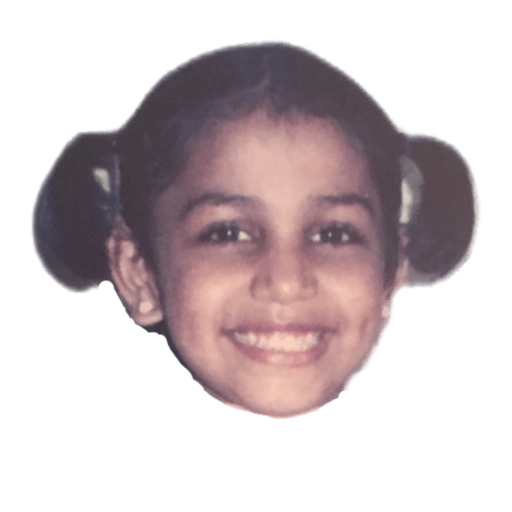
\includegraphics[width=10cm]{"images/experiment_5/error_main.png"}
    %             \caption{Main Sources of error }
    %             \label{fig:Main_error_chap_5}
    %         \end{figure}
    
    \section{Data Collection \& Pose Filtering}
    \begin{itemize}
        \item The placement experiment with KUKA youBot arm was carried out for 20 times in the straight, left and right directions using small, medium and large objects. Therefore each team collected a total of atleast a total of 180 readings.
        \item Compared to the data collected from the LEGO experiment, the data collected from this experiment was found to be more visually consistent and has fewer outliers. Tables \ref{tab:large-object}, \ref{tab:medium-object} \& \ref{tab:small-object} represent the data of object poses collected by our group using the Largee, Medium and Small objects, for each direction. The coordinates, x \& y were converted to centimeters from meters and the angles were converted from radians to degrees.
        \item The Figure \ref{fig:exp05-test-set-up} shows the camera and robot set up used for the experiment. After placing the object on the container the robot performs the motion on command. At the end of each motion the user run a python code to collect pose of the object and the 
        \begin{figure}[H] 
            \centering 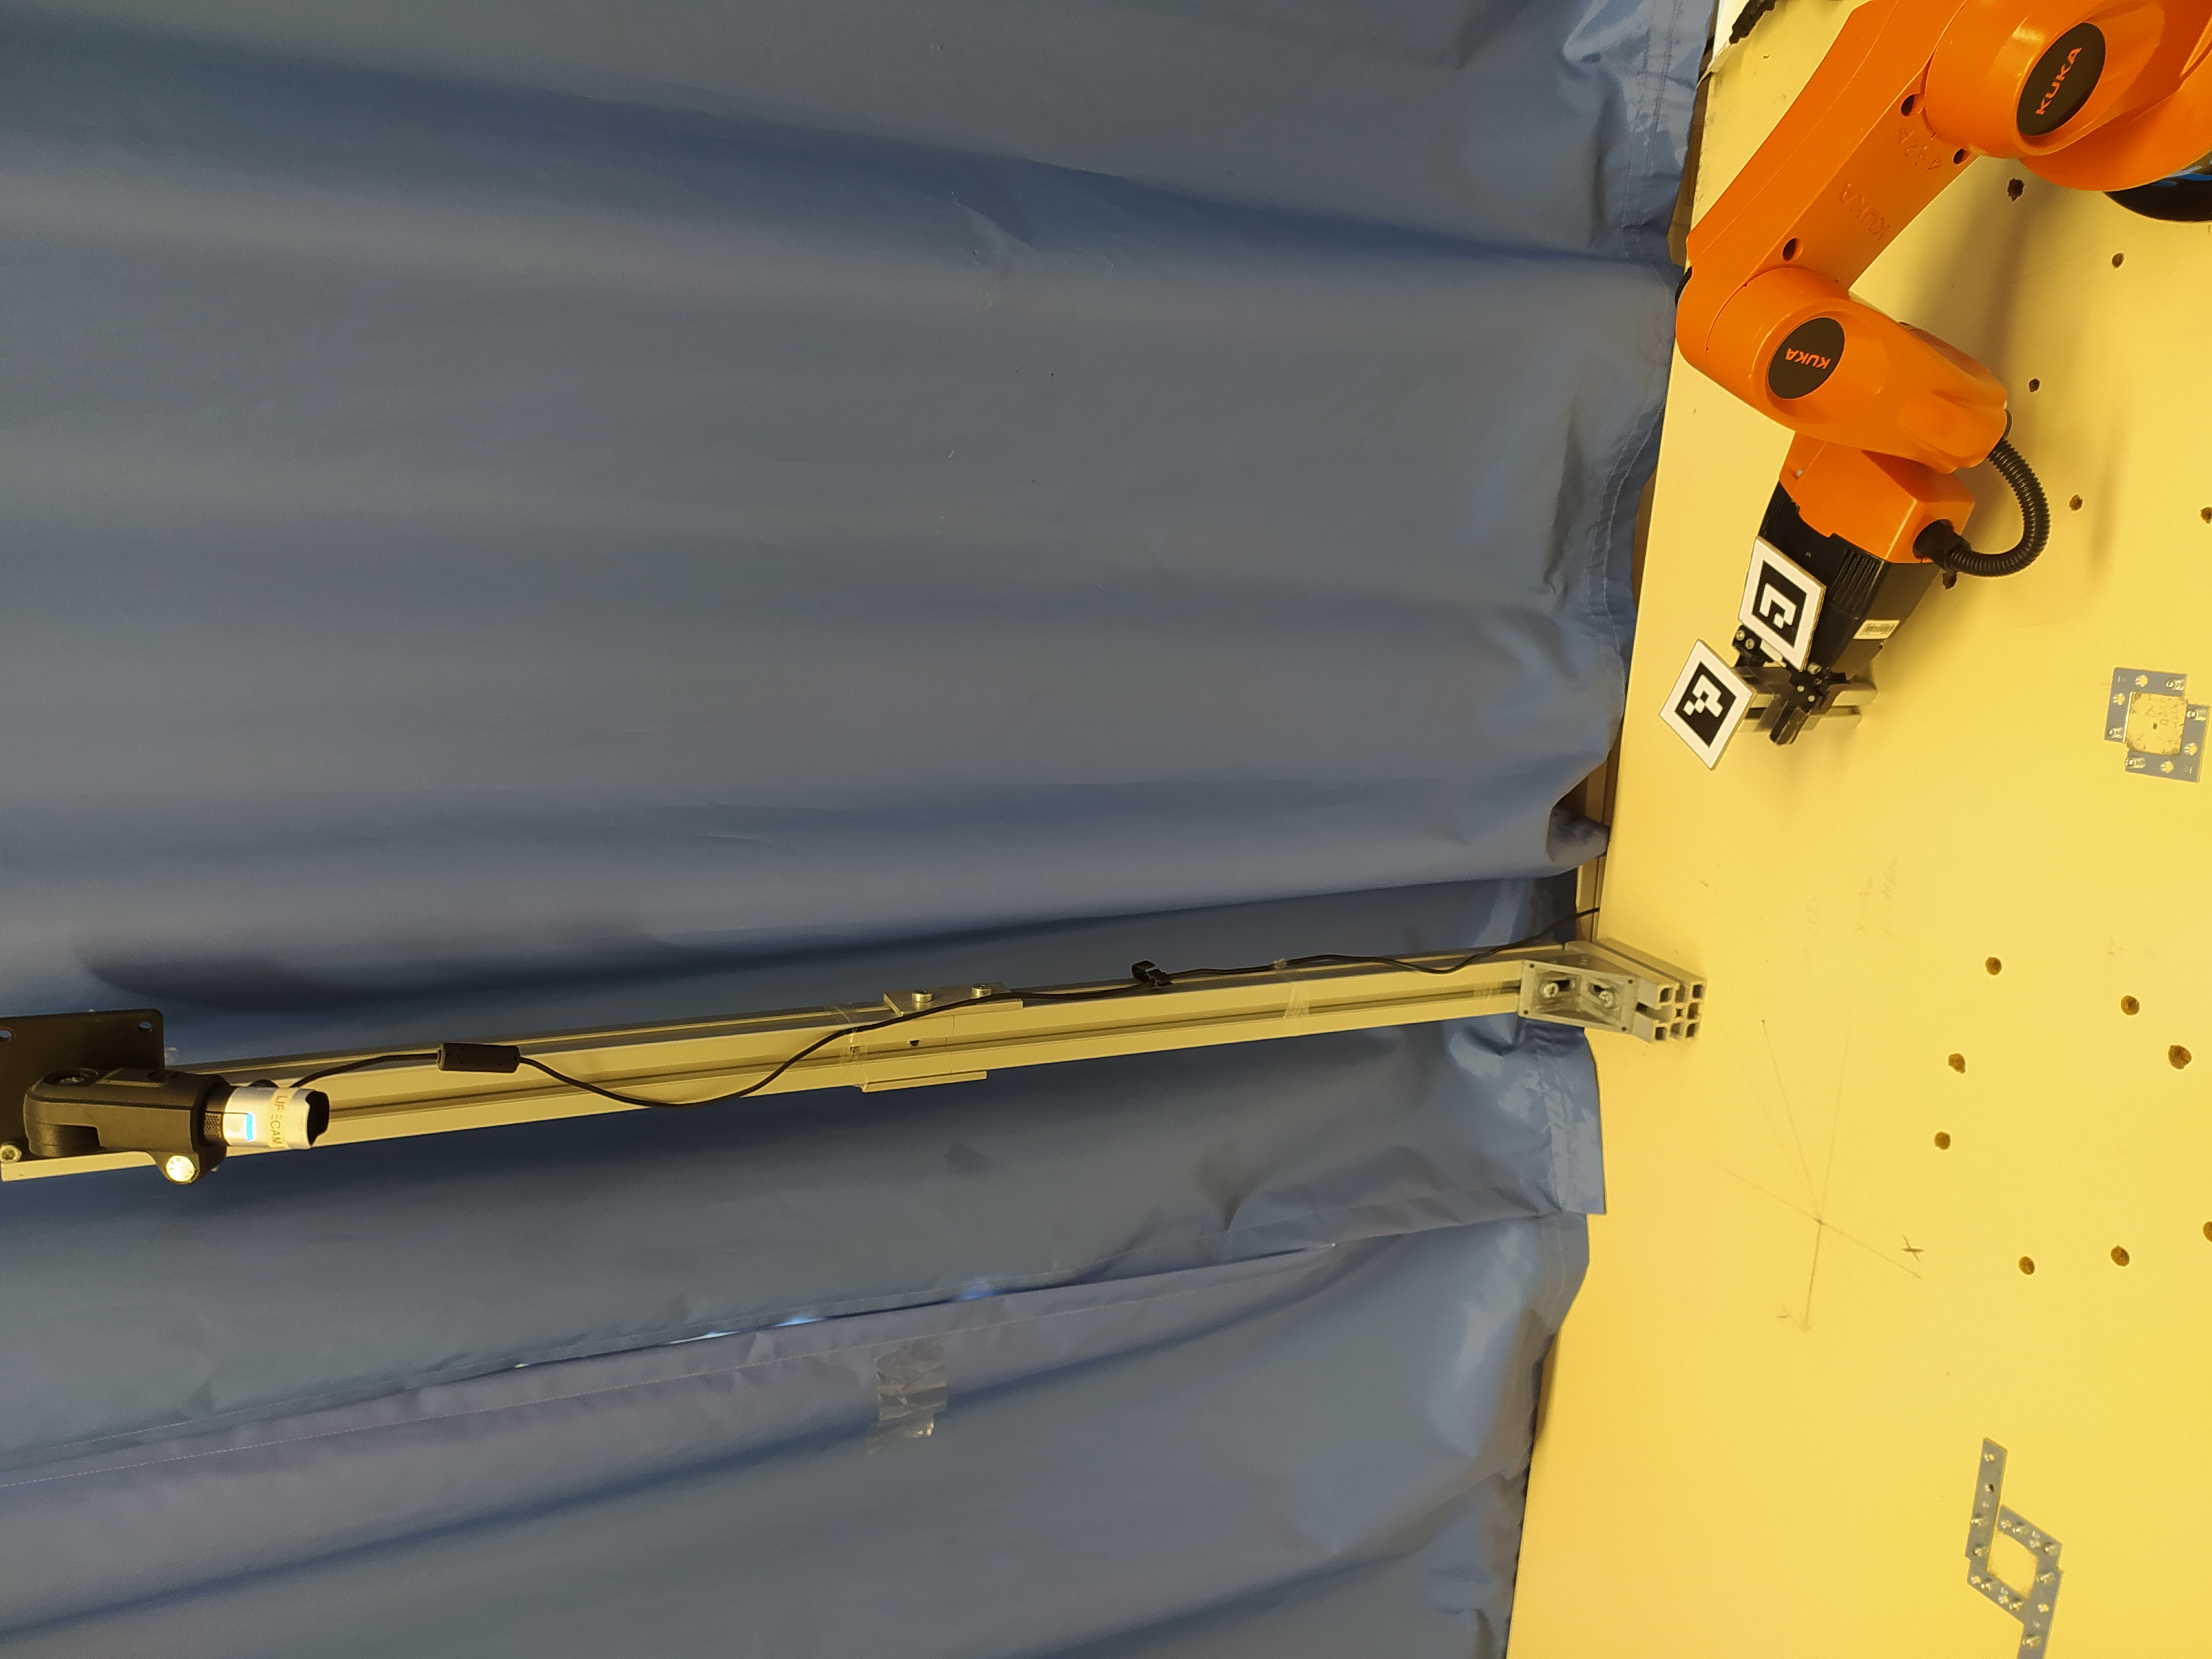
\includegraphics[width=\textwidth]{"images/experiment_5/camera_system.jpg"}
            \caption{{Test set up}}
            \label{fig:exp05-test-set-up}
        \end{figure}
        \item The world coordinate system was defined from the hand drawn coordinates as depicted in Figure \ref{fig:exp05-coordinate-world}
        
        
        \begin{figure}[H] 
            \centering 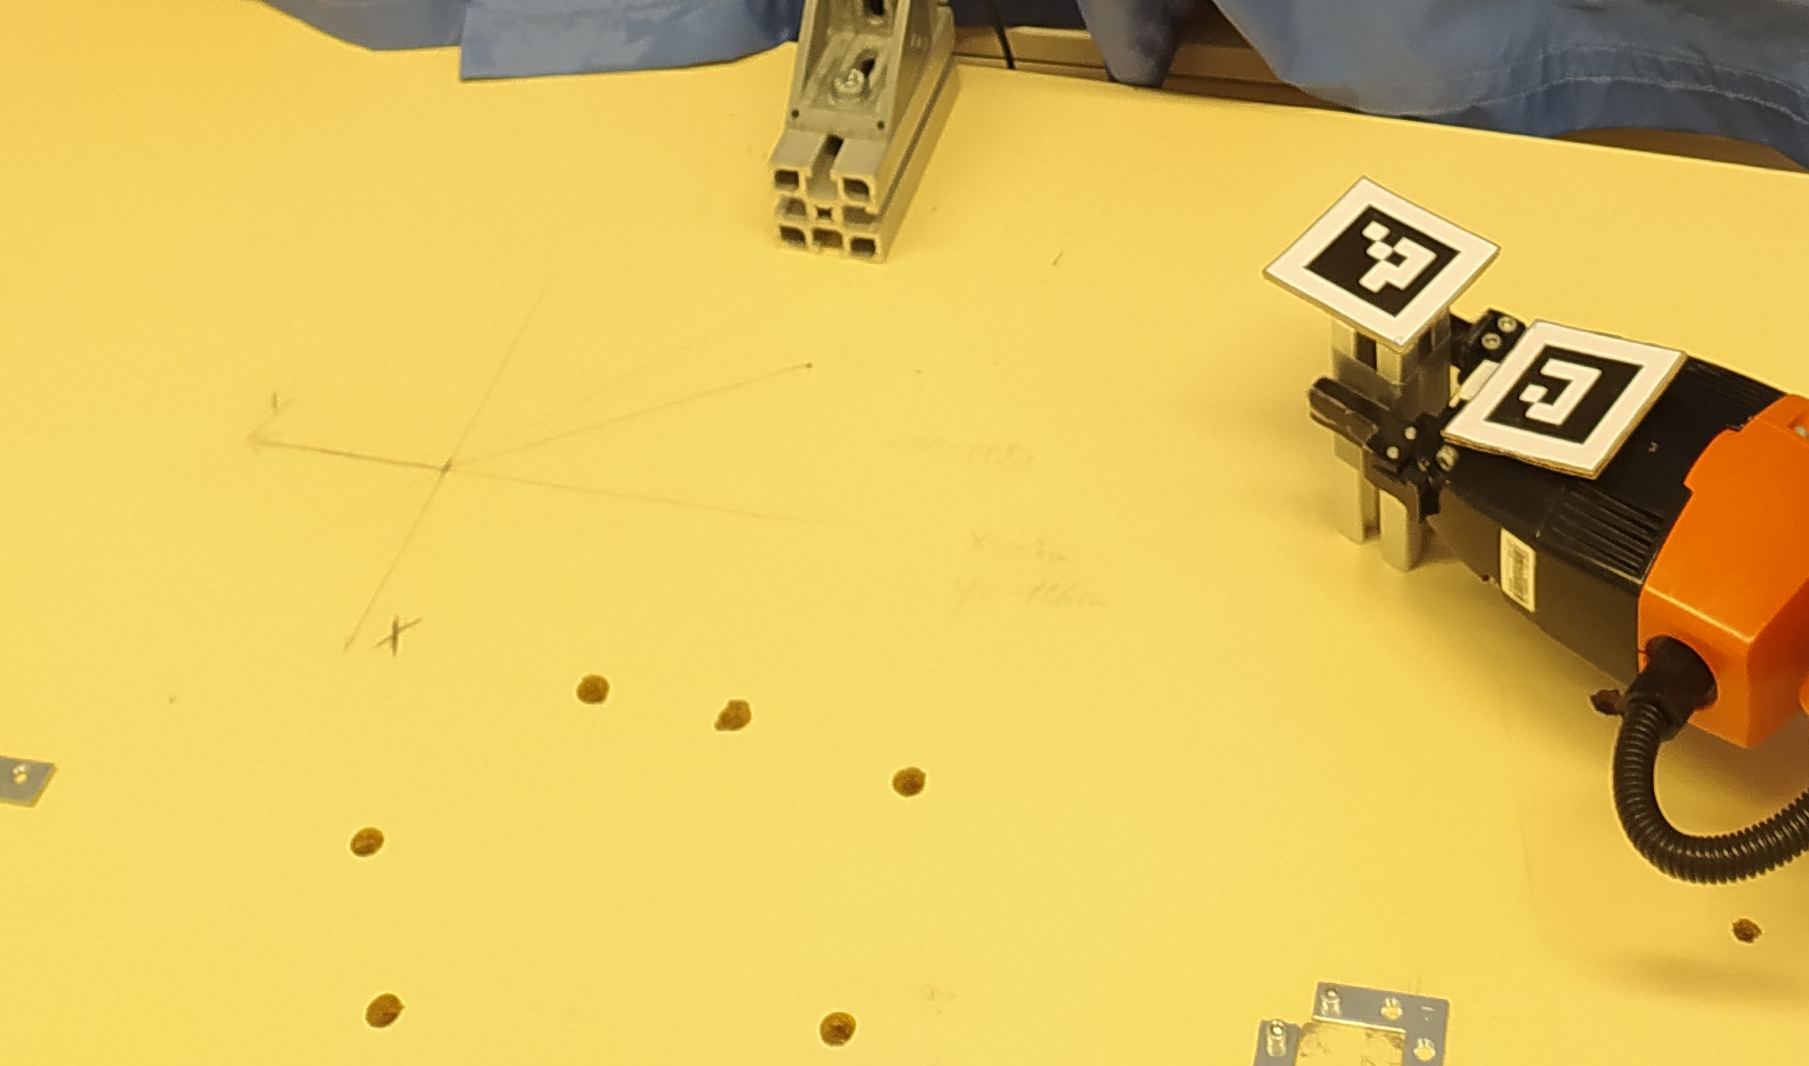
\includegraphics[width=\textwidth]{"images/experiment_5/Coordinate_system.png"}
            \caption{{World Coordinate}}
            \label{fig:exp05-coordinate-world}
        \end{figure}
        
        
           
        \item Given below in table \ref{tab:outliers_chapter5}, is a summary of the outliers found using the Chebyshev outlier detection method where we removed points outside two standard deviations. We used the data from all the groups.
        \item \textcolor{blue}{When performing outlier for removal for both end effector and object poses we removed the entire data point if either of position values(x or y coordinate) or orientation value was outside two standard deviations. The outlier removal was perfomed after taking the average of the 50 data readings per pose given by the camera system} 
    \end{itemize}

\begin{table}[]
\centering
\resizebox{\textwidth}{!}{%
\begin{tabular}{|r|r|r|r|r|r|r|r|r|r|}
\hline
\multicolumn{1}{|l|}{}        & \multicolumn{3}{c|}{Straight}                                                                      & \multicolumn{3}{c|}{Right}                                                                         & \multicolumn{3}{c|}{Left}                                                                          \\ \hline
\multicolumn{1}{|l|}{Sl. No.} & \multicolumn{1}{l|}{x (cm)} & \multicolumn{1}{l|}{y (cm)} & \multicolumn{1}{l|}{Orientation (deg)} & \multicolumn{1}{l|}{x (cm)} & \multicolumn{1}{l|}{y (cm)} & \multicolumn{1}{l|}{Orientation (deg)} & \multicolumn{1}{l|}{x (cm)} & \multicolumn{1}{l|}{y (cm)} & \multicolumn{1}{l|}{Orientation (deg)} \\ \hline
1                             & 16.40                        & -20.83                      & -92.97                                 & -4.80                        & -34.55                      & -63.69                                 & 35.65                       & -27.36                      & -118.53                                \\ \hline
2                             & 16.42                       & -20.91                      & -94.81                                 & -4.80                        & -34.55                      & -63.72                                 & 35.71                       & -27.38                      & -118.77                                \\ \hline
3                             & 16.27                       & -20.79                      & -92.8                                  & -4.84                       & -34.15                      & -63.79                                 & 35.92                       & -27.44                      & -119.71                                \\ \hline
4                             & 16.71                       & -21.06                      & -93.3                                  & -4.91                       & -34.55                      & -63.69                                 & 35.5                        & -27.30                       & -118.54                                \\ \hline
5                             & 16.41                       & -20.87                      & -92.88                                 & -4.92                       & -34.35                      & -64.54                                 & 36.26                       & -27.68                      & -116.6                                 \\ \hline
6                             & 16.61                       & -21.17                      & -93.25                                 & -4.95                       & -34.71                      & -62.36                                 & 35.50                        & -27.30                       & -118.54                                \\ \hline
7                             & 16.66                       & -21.01                      & -92.10                                  & -4.73                       & -34.37                      & -67.13                                 & 35.09                       & -27.13                      & -117.36                                \\ \hline
8                             & 16.36                       & -20.84                      & -92.99                                 & -4.85                       & -34.75                      & -61.17                                 & 35.6                        & -27.34                      & -118.70                                 \\ \hline
9                             & 16.42                       & -20.78                      & -94.78                                 & 36.14                       & -27.51                      & -117.96                                & 36.05                       & -27.59                      & -116.48                                \\ \hline
10                            & 16.45                       & -20.80                       & -94.69                                 & -4.82                       & -34.28                      & -63.14                                 & 35.6                        & -27.34                      & -118.60                                 \\ \hline
11                            & 16.66                       & -21.00                         & -92.12                                 & -4.88                       & -34.34                      & -64.14                                 & 35.66                       & -27.41                      & -115.79                                \\ \hline
12                            & 16.59                       & -20.95                      & -93.87                                 & -4.80                        & -34.57                      & -64.1                                  & 35.60                        & -27.35                      & -118.58                                \\ \hline
13                            & 16.25                       & -20.81                      & -94.42                                 & -4.89                       & -34.74                      & -62.77                                 & 35.53                       & -27.33                      & -118.33                                \\ \hline
14                            & 16.51                       & -20.94                      & -94.59                                 & -4.80                        & -34.55                      & -63.72                                 & 35.13                       & -27.14                      & -117.45                                \\ \hline
15                            & 16.48                       & -20.96                      & -93.04                                 & -4.84                       & -34.29                      & -62.78                                 & 35.54                       & -27.31                      & -118.65                                \\ \hline
16                            & 16.64                       & -20.93                      & -93.77                                 & -4.92                       & -34.55                      & -63.16                                 & 36.15                       & -27.63                      & -116.54                                \\ \hline
17                            & 16.38                       & -20.84                      & -97.93                                 & -4.77                       & -34.42                      & -63.93                                 & 35.41                       & -27.26                      & -118.16                                \\ \hline
18                            & 16.42                       & -20.78                      & -94.78                                 & -4.91                       & -34.56                      & -63.69                                 & 34.87                       & -27.08                      & -119.78                                \\ \hline
19                            & 16.51                       & -20.96                      & -90.03                                 & -4.79                       & -34.5                       & -63.96                                 & 35.51                       & -27.30                       & -118.54                                \\ \hline
20                            & 16.42                       & -20.78                      & -94.78                                 & -4.91                       & -34.29                      & -64.99                                 & 36.00                          & -27.55                      & -117.05                                \\ \hline
\end{tabular}%
}
\caption{\textcolor{blue}{Object pose data collected for the Large Object}}
\label{tab:large-object}
\end{table}

\begin{table}[]
\centering
\resizebox{\textwidth}{!}{%
\begin{tabular}{|c|r|r|r|r|r|r|r|r|r|}
\hline
        & \multicolumn{3}{c|}{Straight}                                                                      & \multicolumn{3}{c|}{Right}                                                                         & \multicolumn{3}{c|}{Left}                                                                          \\ \hline
Sl. No. & \multicolumn{1}{c|}{x (cm)} & \multicolumn{1}{c|}{y (cm)} & \multicolumn{1}{c|}{Orientation (deg)} & \multicolumn{1}{c|}{x (cm)} & \multicolumn{1}{c|}{y (cm)} & \multicolumn{1}{c|}{Orientation (deg)} & \multicolumn{1}{c|}{x (cm)} & \multicolumn{1}{c|}{y (cm)} & \multicolumn{1}{c|}{Orientation (deg)} \\ \hline
1       & 16.30                        & -20.68                      & -96.57                                 & -5.17                       & -34.29                      & -64.28                                 & 35.16                       & -27.31                      & -117.95                                \\ \hline
2       & 16.65                       & -20.43                      & -95.62                                 & -5.16                       & -34.31                      & -64.39                                 & 35.88                       & -27.28                      & -115.11                                \\ \hline
3       & 16.66                       & -20.64                      & -97.1                                  & -5.09                       & -34.13                      & -64.68                                 & 34.98                       & -27.11                      & -109.79                                \\ \hline
4       & 16.33                       & -20.55                      & -96.56                                 & -5.20                        & -34.34                      & -61.43                                 & 35.38                       & -27.36                      & -109.64                                \\ \hline
5       & 16.39                       & -20.5                       & -94.66                                 & -5.10                        & -34.08                      & -64.47                                 & 35.22                       & -27.30                       & -117.89                                \\ \hline
6       & 16.45                       & -20.66                      & -92.03                                 & -5.10                        & -34.35                      & -61.34                                 & 35.22                       & -27.31                      & -117.92                                \\ \hline
7       & 16.61                       & -20.80                       & -93.60                                  & -5.14                       & -34.09                      & -66.62                                 & 35.70                        & -27.30                       & -107.1                                 \\ \hline
8       & 16.40                        & -20.61                      & -94.15                                 & -5.10                        & -34.10                       & -64.48                                 & 35.81                       & -26.94                      & -118.95                                \\ \hline
9       & 16.33                       & -20.56                      & -92.83                                 & -5.14                       & -34.39                      & -62.82                                 & 35.61                       & -26.97                      & -123.67                                \\ \hline
10      & 16.53                       & -20.43                      & -93.4                                  & -5.22                       & -34.59                      & -60.79                                 & 35.13                       & -27.29                      & -117.97                                \\ \hline
11      & 16.30                        & -20.28                      & -101.92                                & -5.11                       & -34.15                      & -64.38                                 & 35.69                       & -27.03                      & -122.76                                \\ \hline
12      & 16.46                       & -21.09                      & -96.03                                 & -5.15                       & -34.52                      & -61.48                                 & 35.40                        & -27.21                      & -117.78                                \\ \hline
13      & 16.14                       & -20.24                      & -93.65                                 & -5.11                       & -34.23                      & -64.46                                 & 35.25                       & -27.29                      & -117.96                                \\ \hline
14      & 16.62                       & -21.07                      & -93.74                                 & -5.14                       & -34.38                      & -66.50                                  & 35.64                       & -27.43                      & -116.44                                \\ \hline
15      & 16.35                       & -20.27                      & -96.50                                  & -5.21                       & -34.64                      & -63.14                                 & 35.81                       & -27.31                      & -115.72                                \\ \hline
16      & 16.78                       & -20.70                       & -96.82                                 & -5.17                       & -34.61                      & -64.46                                 & 35.24                       & -27.17                      & -117.57                                \\ \hline
17      & 16.14                       & -20.76                      & -93.42                                 & -5.19                       & -34.56                      & -62.85                                 & 36.06                       & -27.53                      & -113.89                                \\ \hline
18      & 16.31                       & -20.74                      & -94.54                                 & -5.15                       & -34.39                      & -64.38                                 & 34.86                       & -27.18                      & -116.65                                \\ \hline
19      & 16.58                       & -20.78                      & -93.45                                 & -5.17                       & -34.27                      & -61.37                                 & 36.05                       & -27.52                      & -113.91                                \\ \hline
20      & 16.32                       & -20.50                       & -91.11                                 & -5.13                       & -33.66                      & -61.66                                 & 35.40                        & -27.36                      & -117.85                                \\ \hline
\end{tabular}%
}
\caption{\textcolor{blue}{Object pose data collected for the Medium Object}}
\label{tab:medium-object}
\end{table}


\begin{table}[]
\centering
\resizebox{\textwidth}{!}{%
\begin{tabular}{|r|r|r|r|r|r|r|r|r|r|}
\hline
\multicolumn{1}{|l|}{}        & \multicolumn{3}{c|}{Straight}                                                                      & \multicolumn{3}{c|}{Right}                                                                         & \multicolumn{3}{c|}{Left}                                                                          \\ \hline
\multicolumn{1}{|l|}{Sl. No.} & \multicolumn{1}{l|}{x (cm)} & \multicolumn{1}{l|}{y (cm)} & \multicolumn{1}{l|}{Orientation (deg)} & \multicolumn{1}{l|}{x (cm)} & \multicolumn{1}{l|}{y (cm)} & \multicolumn{1}{l|}{Orientation (deg)} & \multicolumn{1}{l|}{x (cm)} & \multicolumn{1}{l|}{y (cm)} & \multicolumn{1}{l|}{Orientation (deg)} \\ \hline
1                             & 16.16                       & -21.30                       & -93.49                                 & -5.75                       & -34.61                      & -64.15                                 & 34.77                       & -27.50                       & -117.85                                \\ \hline
2                             & 15.78                       & -21.14                      & -92.68                                 & -5.68                       & -34.82                      & -64.08                                 & 34.85                       & -27.43                      & -117.39                                \\ \hline
3                             & 15.62                       & -20.94                      & -93.23                                 & -5.74                       & -34.63                      & -63.69                                 & 34.55                       & -27.44                      & -117.41                                \\ \hline
4                             & 16.16                       & -21.3                       & -93.49                                 & -5.74                       & -34.95                      & -60.28                                 & 34.83                       & -27.49                      & -118.01                                \\ \hline
5                             & 15.78                       & -21.14                      & -92.68                                 & -5.62                       & -34.68                      & -63.04                                 & 34.74                       & -27.53                      & -117.97                                \\ \hline
6                             & 15.74                       & -20.99                      & -92.79                                 & -5.71                       & -35.01                      & -63.85                                 & 36.04                       & -28.00                         & -117.97                                \\ \hline
7                             & 15.54                       & -20.91                      & -93.55                                 & -5.81                       & -34.89                      & -63.82                                 & 35.20                        & -27.57                      & -119.44                                \\ \hline
8                             & 15.78                       & -21.14                      & -92.68                                 & -5.73                       & -34.99                      & -60.13                                 & 34.59                       & -27.41                      & -117.49                                \\ \hline
9                             & 16.16                       & -21.30                       & -93.49                                 & -5.74                       & -34.93                      & -60.52                                 & 34.29                       & -27.30                       & -116.73                                \\ \hline
10                            & 15.96                       & -21.22                      & -93.06                                 & -5.74                       & -34.76                      & -62.33                                 & 35.56                       & -27.76                      & -116.72                                \\ \hline
11                            & 15.73                       & -21.03                      & -94.16                                 & -5.73                       & -34.76                      & -62.26                                 & 34.74                       & -27.53                      & -117.97                                \\ \hline
12                            & 16.00                          & -21.23                      & -93.15                                 & -5.76                       & -35.08                      & -58.21                                 & 34.74                       & -27.53                      & -117.97                                \\ \hline
13                            & 16.16                       & -21.30                       & -93.49                                 & -5.76                       & -35.08                      & -58.30                                  & 35.28                       & -27.66                      & -114.62                                \\ \hline
14                            & 15.78                       & -21.14                      & -92.68                                 & -5.74                       & -34.58                      & -63.87                                 & 36.04                       & -28.00                         & -117.97                                \\ \hline
15                            & 15.78                       & -21.14                      & -92.68                                 & -5.74                       & -34.59                      & -64.14                                 & 34.38                       & -27.35                      & -116.93                                \\ \hline
16                            & 15.79                       & -21.14                      & -92.70                                  & -5.66                       & -35.00                         & -62.4                                  & 34.98                       & -27.57                      & -118.4                                 \\ \hline
17                            & 15.75                       & -21.05                      & -94.25                                 & -5.76                       & -34.67                      & -63.89                                 & 35.13                       & -27.64                      & -118.76                                \\ \hline
18                            & 15.78                       & -21.06                      & -94.33                                 & -5.73                       & -34.70                       & -62.50                                  & 35.53                       & -27.75                      & -117.51                                \\ \hline
19                            & 15.83                       & -21.08                      & -94.37                                 & -5.73                       & -35.02                      & -61.87                                 & 34.74                       & -27.53                      & -117.97                                \\ \hline
20                            & 15.58                       & -20.93                      & -93.73                                 & -5.62                       & -34.72                      & -62.57                                 & 35.00                          & -27.50                       & -117.73                                \\ \hline
\end{tabular}%
}
\caption{\textcolor{blue}{Object pose data collected for the Small Object}}
\label{tab:small-object}
\end{table}



%The end effector posee

% Large Object
\begin{table}[]
\centering
\begin{tabular}{|l|l|l|r|l|l|r|l|l|r|}
\hline
                               & \multicolumn{3}{l|}{\textbf{Straight}} & \multicolumn{3}{l|}{\textbf{Left}} & \multicolumn{3}{l|}{\textbf{Right}} \\ \cline{2-10} 
\multirow{-2}{*}{\textbf{SI No}} & x(cm)           & y(cm)            & Orientation(deg)          & x(cm)  & y(cm)  & Orientation(deg) & x(cm)  & y(cm)   & Orientation(deg) \\ \hline
1                                                        & 17.31           & -29.99           & -5.29                     & 33.48  & -36.57 & -28.15           & -0.57  & -41.24  & 20.34            \\ \hline
2                                                        & 17.31           & -29.99           & -5.29                     & 33.48  & -36.57 & -28.15           & -0.57  & -41.20  & 20.59            \\ \hline
3                                                        & 17.41           & -30.08           & -4.59                     & 33.45  & -36.56 & -28.56           & -0.57  & -41.20  & 20.59            \\ \hline
4                                                        & 17.35           & -30.03           & -5.10                     & 33.48  & -36.57 & -28.15           & -0.57  & -41.54  & 19.30            \\ \hline
5                                                        & 17.31           & -29.99           & -5.29                     & 33.47  & -36.55 & -28.21           & -0.57  & -41.21  & 20.57            \\ \hline
6                                                        & 17.32           & -29.99           & -5.25                     & 33.48  & -36.57 & -28.16           & -0.57  & -41.26  & 20.27            \\ \hline
7                                                        & 17.31           & -29.99           & -5.29                     & 33.48  & -36.57 & -28.15           & -0.57  & -41.22  & 20.55            \\ \hline
8                                                        & 17.31           & -29.99           & -5.29                     & 33.48  & -36.57 & -28.15           & -0.56  & -41.24  & 20.54            \\ \hline
9                                                        & 17.31           & -29.99           & -5.29                     & 33.48  & -36.56 & -28.19           & -0.57  & -41.21  & 20.57            \\ \hline
10                                                       & 17.31           & -29.99           & -5.29                     & 33.48  & -36.57 & -28.15           & -0.56  & -41.25  & 20.52            \\ \hline
11                                                       & 17.31           & -29.99           & -5.29                     & 33.41  & -36.52 & -28.31           & -0.57  & -41.21  & 20.57            \\ \hline
12                                                       & 17.34           & -30.02           & -5.14                     & 33.48  & -36.57 & -28.15           & -0.57  & -41.26  & 20.22            \\ \hline
13                                                       & 17.31           & -29.99           & -5.29                     & 33.44  & -36.56 & -28.56           & -0.56  & -41.24  & 20.54            \\ \hline
14                                                       & 17.31           & -29.99           & -5.29                     & 33.48  & -36.57 & -28.15           & -0.57  & -41.31  & 20.06            \\ \hline
15                                                       & 17.31           & -29.99           & -5.29                     & 33.46  & -36.56 & -28.41           & -0.56  & -41.30  & 20.45            \\ \hline
16                                                       & 17.58           & -30.25           & -3.46                     & 33.48  & -36.57 & -28.15           & -0.57  & -41.21  & 20.57            \\ \hline
17                                                       & 17.31           & -29.99           & -5.29                     & 33.48  & -36.56 & -28.21           & -0.57  & -41.25  & 20.35            \\ \hline
18                                                       & 17.52           & -30.20           & -4.08                     & 33.46  & -36.56 & -28.41           & -0.57  & -41.39  & 19.33            \\ \hline
19                                                       & 17.31           & -29.99           & -5.29                     & 33.46  & -36.55 & -28.29           & -0.56  & -41.24  & 20.49            \\ \hline
20                                                       & 17.31           & -29.99           & -5.29                     & 33.44  & -36.56 & -28.60           & -0.56  & -41.27  & 20.50            \\ \hline
\end{tabular}
\caption{\textcolor{blue}{End effector pose data collected for the Large Object}}
\label{tab:ee-large-object}
\end{table}

%Medium end effecto

\begin{table}[] \footnotesize
\centering
\begin{tabular}{|l|l|l|r|l|l|r|l|l|r|}
\hline
                                & \multicolumn{3}{l|}{\textbf{Straight}} & \multicolumn{3}{l|}{\textbf{Left}} & \multicolumn{3}{l|}{\textbf{Right}} \\ \cline{2-10} 
\multirow{-2}{*}{\textbf{SI No}} & x(cm)           & y(cm)            & Orientation(deg)          & x(cm)  & y(cm)  & Orientation(deg) & x(cm)  & y(cm)   & Orientation(deg) \\ \hline
1                                                        & 17.37           & -30.02           & -4.52                     & 33.48  & -36.57 & -28.15           & -0.56  & -41.31  & 20.44            \\ \hline
2                                                        & 17.37           & -30.02           & -4.45                     & 33.48  & -36.57 & -28.15           & -0.57  & -41.22  & 20.55            \\ \hline
3                                                        & 17.38           & -30.02           & -4.58                     & 33.48  & -36.57 & -28.15           & -0.56  & -41.28  & 20.47            \\ \hline
4                                                        & 17.37           & -30.02           & -4.51                     & 33.48  & -36.57 & -28.15           & -0.57  & -41.22  & 20.55            \\ \hline
5                                                        & 17.37           & -30.02           & -4.49                     & 33.48  & -36.57 & -28.15           & -0.56  & -41.32  & 20.42            \\ \hline
6                                                        & 17.35           & -30.01           & -4.78                     & 33.48  & -36.56 & -28.20           & -0.56  & -41.33  & 20.40            \\ \hline
7                                                        & 17.38           & -30.03           & -4.40                     & 33.48  & -36.57 & -28.15           & -0.56  & -41.27  & 20.40            \\ \hline
8                                                        & 17.37           & -30.03           & -4.41                     & 33.48  & -36.57 & -28.15           & -0.57  & -41.22  & 20.52            \\ \hline
9                                                        & 17.37           & -30.03           & -4.41                     & 33.48  & -36.57 & -28.15           & -0.56  & -41.30  & 20.45            \\ \hline
10                                                       & 17.37           & -30.02           & -4.51                     & 33.48  & -36.56 & -28.19           & -0.56  & -41.28  & 20.47            \\ \hline
11                                                       & 17.38           & -30.03           & -4.38                     & 33.47  & -36.56 & -28.29           & -0.56  & -41.28  & 20.47            \\ \hline
12                                                       & 17.38           & -30.03           & -4.40                     & 33.48  & -36.57 & -28.15           & -0.57  & -41.22  & 20.55            \\ \hline
13                                                       & 17.36           & -30.02           & -4.56                     & 33.48  & -36.57 & -28.15           & -0.56  & -41.24  & 20.54            \\ \hline
14                                                       & 17.37           & -30.03           & -4.43                     & 33.47  & -36.56 & -28.26           & -0.53  & -40.20  & 20.47            \\ \hline
15                                                       & 17.38           & -30.03           & -4.38                     & 33.48  & -36.57 & -28.15           & -0.56  & -41.25  & 20.52            \\ \hline
16                                                       & 17.36           & -30.02           & -4.56                     & 33.48  & -36.57 & -28.15           & -0.56  & -41.31  & 20.44            \\ \hline
17                                                       & 17.38           & -30.03           & -4.38                     & 33.48  & -36.57 & -28.16           & -0.56  & -41.30  & 20.45            \\ \hline
18                                                       & 17.36           & -30.02           & -4.54                     & 33.48  & -36.57 & -28.15           & -0.56  & -41.26  & 20.50            \\ \hline
19                                                       & 17.38           & -30.03           & -4.38                     & 33.48  & -36.57 & -28.15           & -0.56  & -41.27  & 20.49            \\ \hline
20                                                       & 17.38           & -30.03           & -4.38                     & 33.48  & -36.57 & -28.15           & -0.56  & -41.24  & 20.54            \\ \hline
\end{tabular}
\caption{\textcolor{blue}{End effector pose data collected for the Medium Object}}
\label{tab:ee-medium-object}
\end{table}



% small end effecot
\begin{table}[]
\centering
\begin{tabular}{|l|l|l|r|l|l|r|l|l|r|}
\hline
                           & \multicolumn{3}{l|}{\textbf{Straight}} & \multicolumn{3}{l|}{\textbf{Left}} & \multicolumn{3}{l|}{\textbf{Right}} \\ \cline{2-10} 
\multirow{-2}{*}{\textbf{}} & x(cm)           & y(cm)            & Orientation(deg)          & x(cm)  & y(cm)  & Orientation(deg) & x(cm)  & y(cm)   & Orientation(deg) \\ \hline
1                                                   & 17.64           & -30.40           & -3.31                     & 32.61  & -35.99 & -29.67           & -0.69  & -41.21  & 20.55            \\ \hline
2                                                   & 17.54           & -30.28           & -4.15                     & 33.31  & -36.51 & -28.83           & -0.68  & -41.42  & 20.72            \\ \hline
3                                                   & 17.49           & -30.23           & -4.51                     & 33.55  & -35.19 & -28.74           & -0.68  & -41.42  & 20.72            \\ \hline
4                                                   & 17.60           & -30.34           & -3.66                     & 33.41  & -36.58 & -28.71           & -0.68  & -41.26  & 20.59            \\ \hline
5                                                   & 17.36           & -30.08           & -5.56                     & 32.56  & -35.95 & -29.73           & -0.68  & -41.26  & 20.59            \\ \hline
6                                                   & 17.62           & -30.37           & -3.52                     & 33.39  & -36.57 & -28.73           & -0.69  & -41.21  & 20.55            \\ \hline
7                                                   & 17.65           & -30.40           & -3.22                     & 32.61  & -35.99 & -29.67           & -0.69  & -41.21  & 20.55            \\ \hline
8                                                   & 17.64           & -30.41           & -3.00                     & 32.56  & -35.95 & -29.73           & -0.68  & -41.39  & 20.69            \\ \hline
9                                                   & 17.60           & -30.35           & -3.62                     & 33.41  & -36.58 & -28.71           & -0.69  & -41.21  & 20.55            \\ \hline
10                                                  & 17.33           & -30.04           & -5.82                     & 33.41  & -36.58 & -28.71           & -0.69  & -41.21  & 20.55            \\ \hline
11                                                  & 17.64           & -30.40           & -3.31                     & 33.41  & -36.58 & -28.71           & -0.69  & -41.21  & 20.55            \\ \hline
12                                                  & 17.64           & -30.39           & -3.36                     & 33.41  & -36.58 & -28.71           & -0.69  & -41.21  & 20.55            \\ \hline
13                                                  & 17.48           & -30.40           & -4.25                     & 32.57  & -35.97 & -29.71           & -0.68  & -41.22  & 20.56            \\ \hline
14                                                  & 17.55           & -30.29           & -4.04                     & 33.31  & -36.51 & -28.83           & -0.68  & -41.27  & 20.59            \\ \hline
15                                                  & 17.65           & -30.40           & -3.17                     & 33.41  & -36.58 & -28.71           & -0.69  & -41.21  & 20.55            \\ \hline
16                                                  & 17.49           & -30.23           & -4.51                     & 33.41  & -36.58 & -28.71           & -0.68  & -41.42  & 20.72            \\ \hline
17                                                  & 17.42           & -30.15           & -5.09                     & 33.41  & -36.58 & -28.71           & -0.68  & -41.42  & 20.71            \\ \hline
18                                                  & 17.64           & -30.41           & -3.07                     & 33.39  & -36.57 & -28.73           & -0.68  & -41.33  & 20.65            \\ \hline
19                                                  & 17.45           & -30.18           & -4.83                     & 32.73  & -36.08 & -29.52           & -0.69  & -41.21  & 20.55            \\ \hline
20                                                  & 17.60           & -30.35           & -3.62                     & 32.56  & -35.95 & -29.73           & -0.68  & -41.32  & 20.64            \\ \hline
\end{tabular}
\caption{\textcolor{blue}{End effector pose data collected for the Small Object}}
\label{tab:ee-small-object}
\end{table}







%End of end effector poses
    
 
\begin{table}[]
\centering
\begin{tabular}{|l|l|l|r|}
\hline
\textbf{Size} & \textbf{Motion} & \textbf{Original data points} & \textbf{Outliers} \\ \hline
                                      & Straight                                & 123                                                   & 8                 \\ \cline{2-4} 
                                      & Left                                    & 123                                                   & 7                 \\ \cline{2-4} 
\multirow{-3}{*}{Large}               & Right                                   & 126                                                   & 3                 \\ \hline
                                      & Straight                                & 123                                                   & 11                \\ \cline{2-4} 
                                      & Left                                    & 123                                                   & 11                \\ \cline{2-4} 
\multirow{-3}{*}{Medium}              & Right                                   & 124                                                   & 12                \\ \hline
                                      & Straight                                & 127                                                   & 6                 \\ \cline{2-4} 
                                      & Left                                    & 123                                                   & 6                 \\ \cline{2-4} 
\multirow{-3}{*}{Small}               & Right                                   & 123                                                   & 12                \\ \hline
\end{tabular}
\caption{Outliers detected in three motion types from combined group data}
\label{tab:outliers_chapter5}
\end{table}
   

  
    \section{Visualisation}
    
    \begin{itemize}
        \item The figures \ref{fig:exp05-straight-end-poses-before}, \ref{fig:exp05-straight-end-poses-after},
        \ref{fig:exp05-right-end-poses-before}, \ref{fig:exp05-right-end-poses-after}, \ref{fig:exp05-left-end-poses-before} \& \ref{fig:exp05-left-end-poses-after} represent the collective end poses of the Large, Medium and Small objects in the straight, right and left directions respectively. 
        \item It was observed that the number of outliers is minimal. The most obvious outlier (Figure \ref{fig:exp05-right-end-poses-before}) was observed for the right motion.
        \item Visually, the measurements from the left motion seem the most precise. 
        \item Visually the large object seems be more precise.(An quantitative evalution will be done in the next report). This could be accounted for the fact that its larger inertia will make it less susceptible to table shakes.
    \end{itemize}
        
    %000000000000000000000000000000000000000000000000000000000000000000000000000000000000%
    
    \clearpage
    % Straight motion
    
      \begin{figure}[H] 
                \centering
                 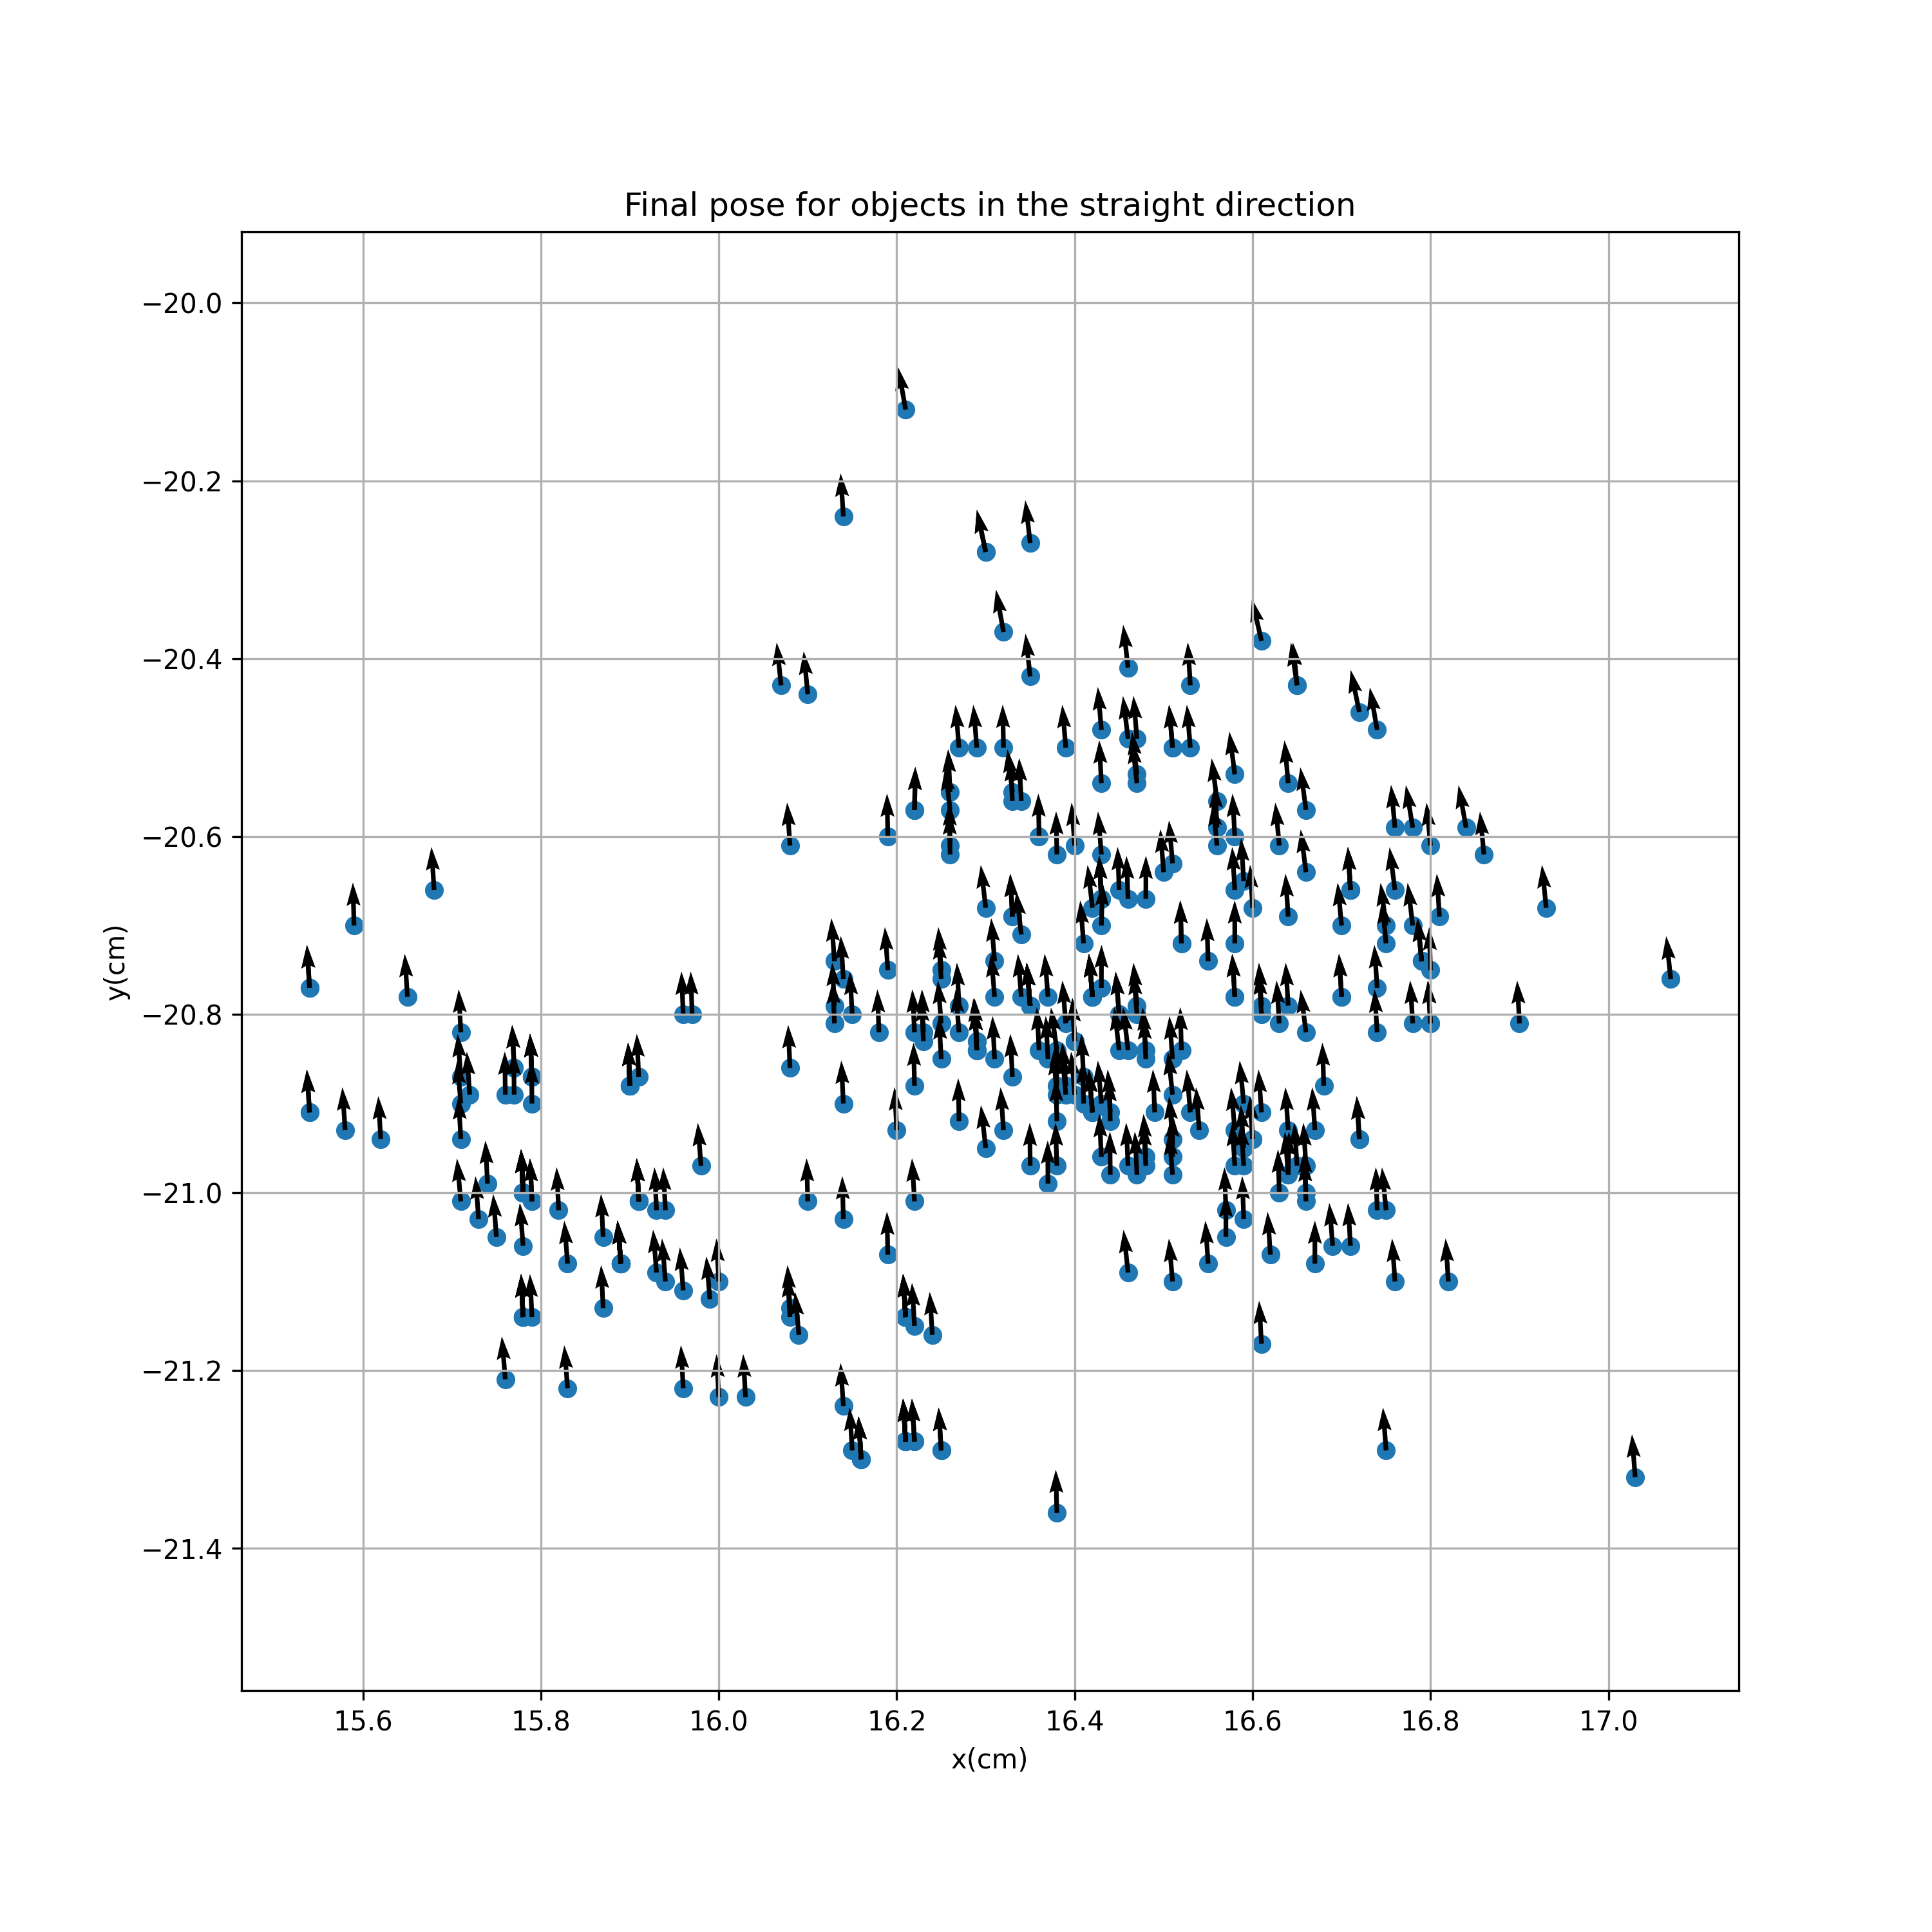
\includegraphics[width=\textwidth]{"images/experiment_5/Final_pose_for_objects_in_the_straight_direction.png"}
                \caption{\textcolor{blue}{Straight motion before removal of outliers(Object Pose)}}
                \label{fig:exp05-straight-end-poses-before}
      \end{figure}
      
      \begin{figure}[H] 
                \centering
                 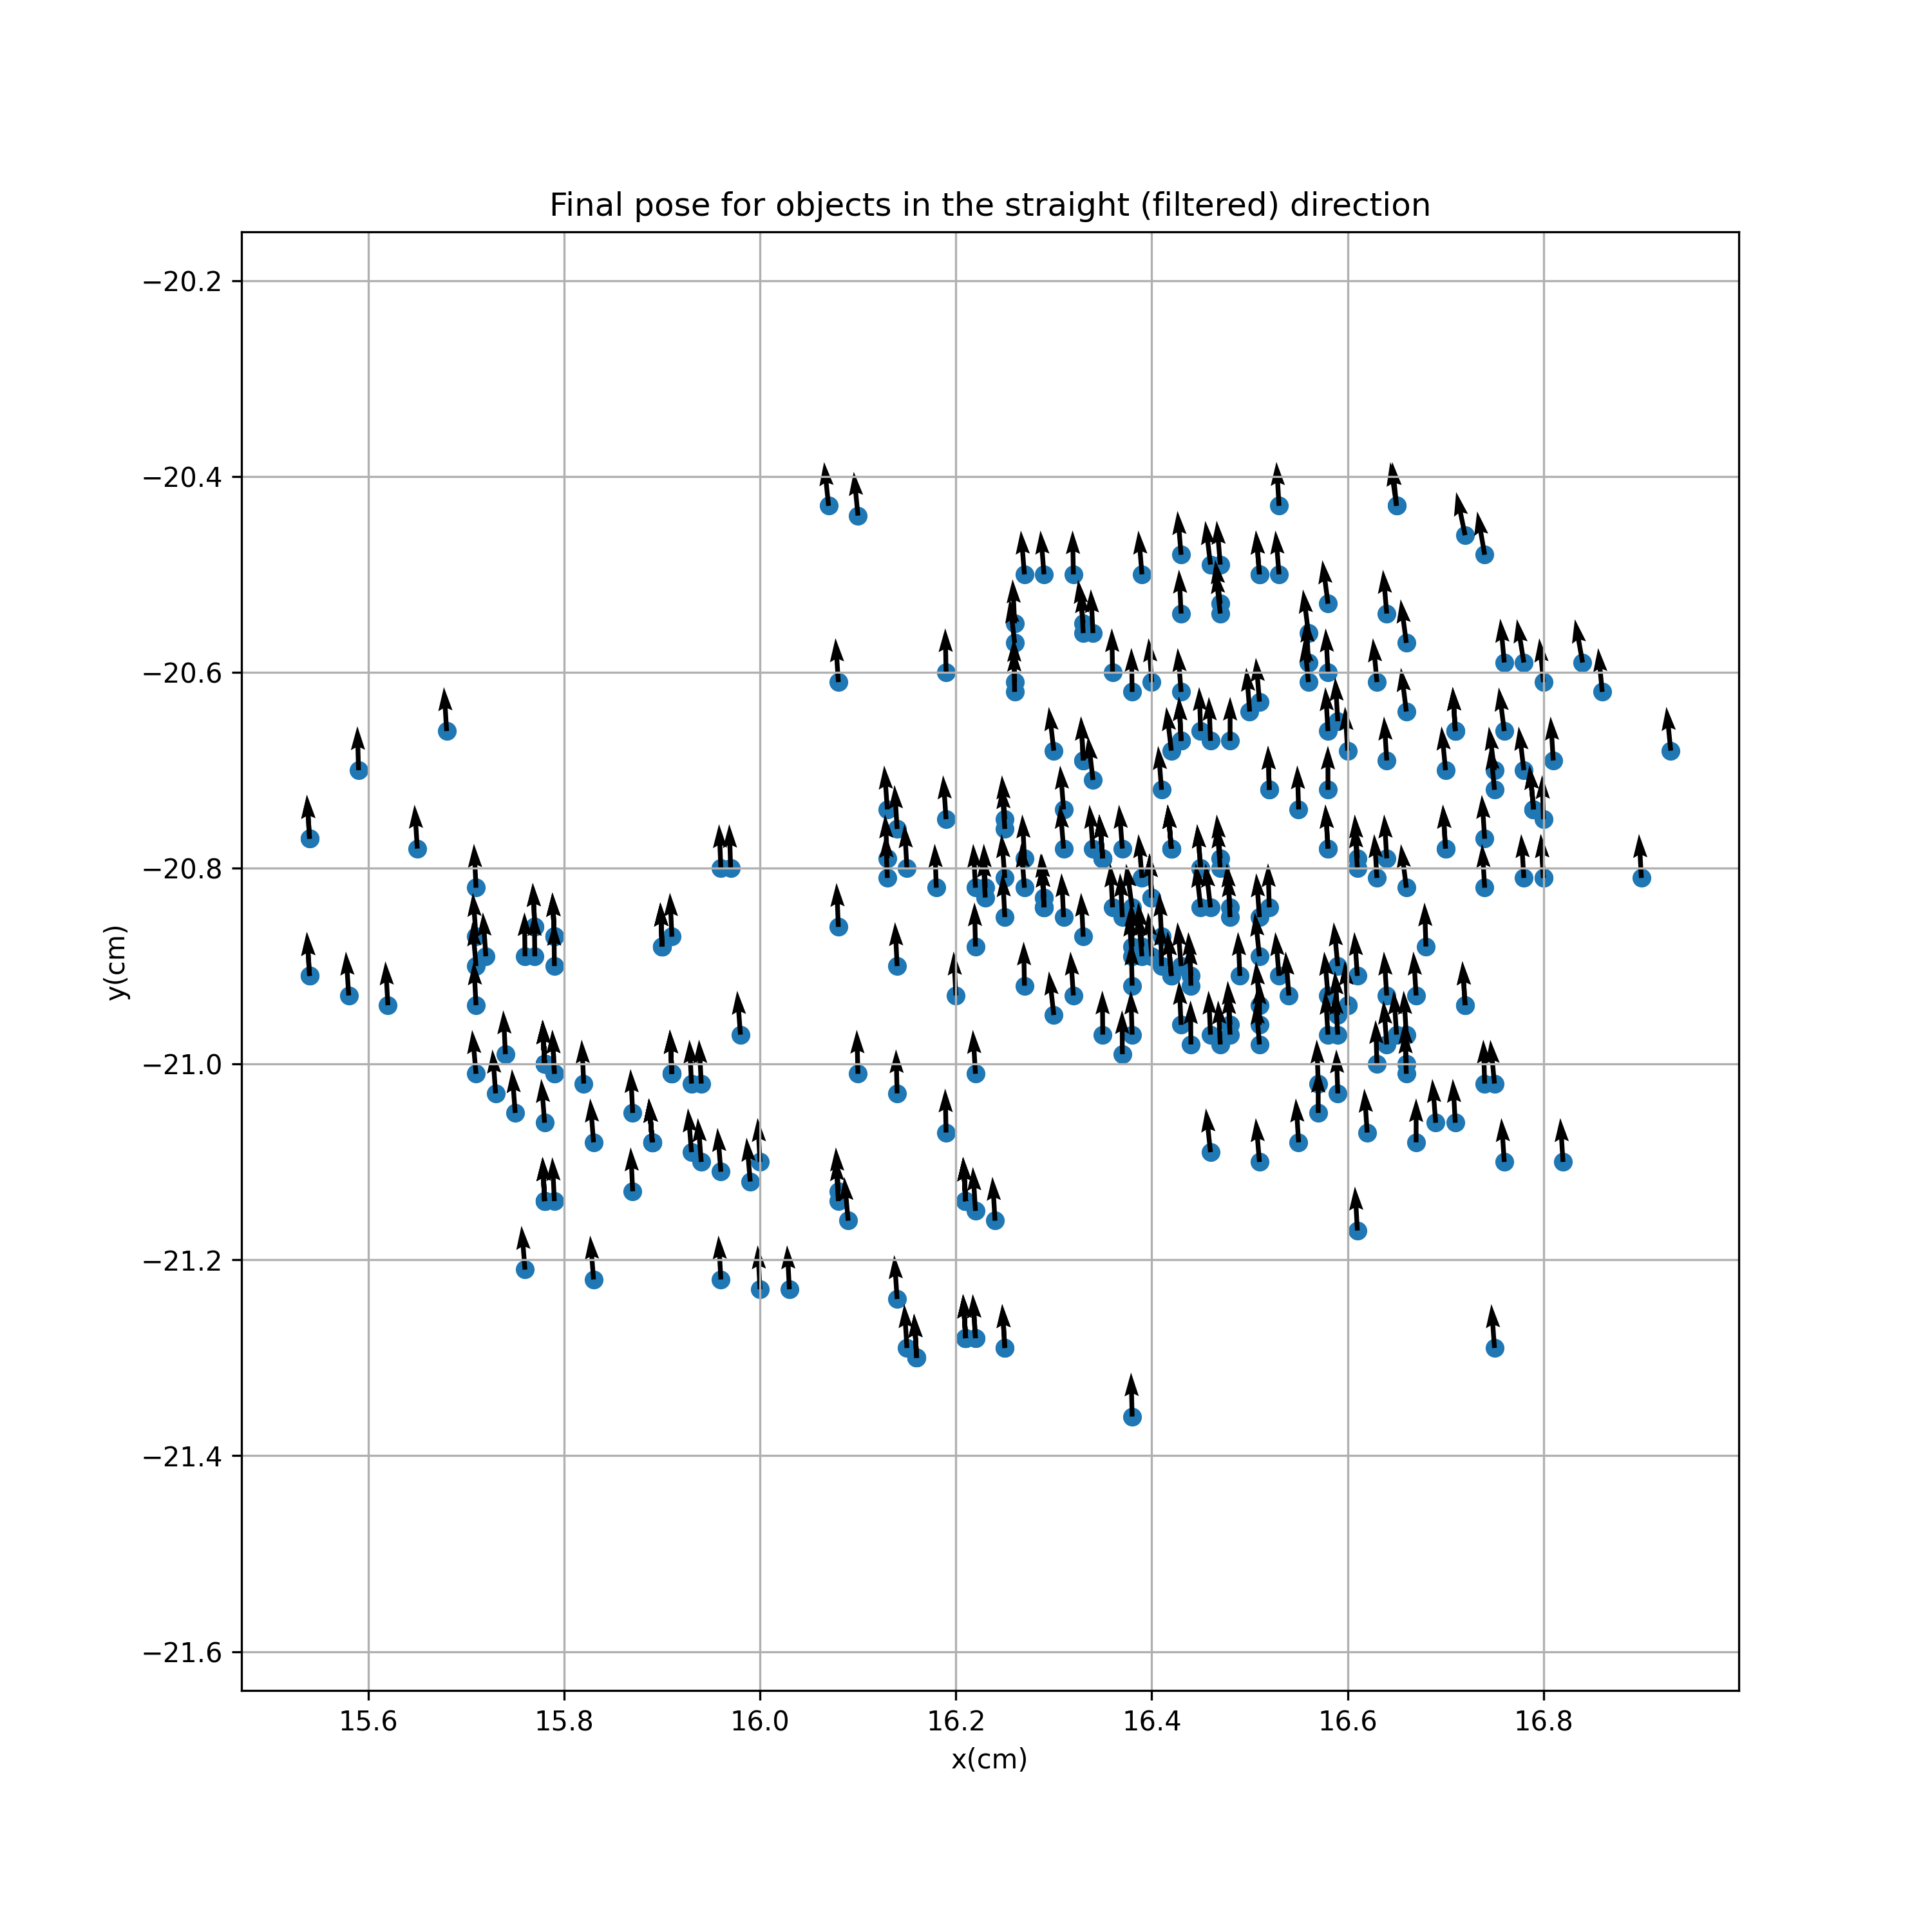
\includegraphics[width=\textwidth]{"images/experiment_5/Final_pose_for_objects_in_the_straight (filtered)_direction.png"}
                \caption{\textcolor{blue}{Straight motion after removal of outliers(Object Pose)}}
                \label{fig:exp05-straight-end-poses-after}
      \end{figure}

    % Left motion

    \begin{figure}[H] 
            \centering 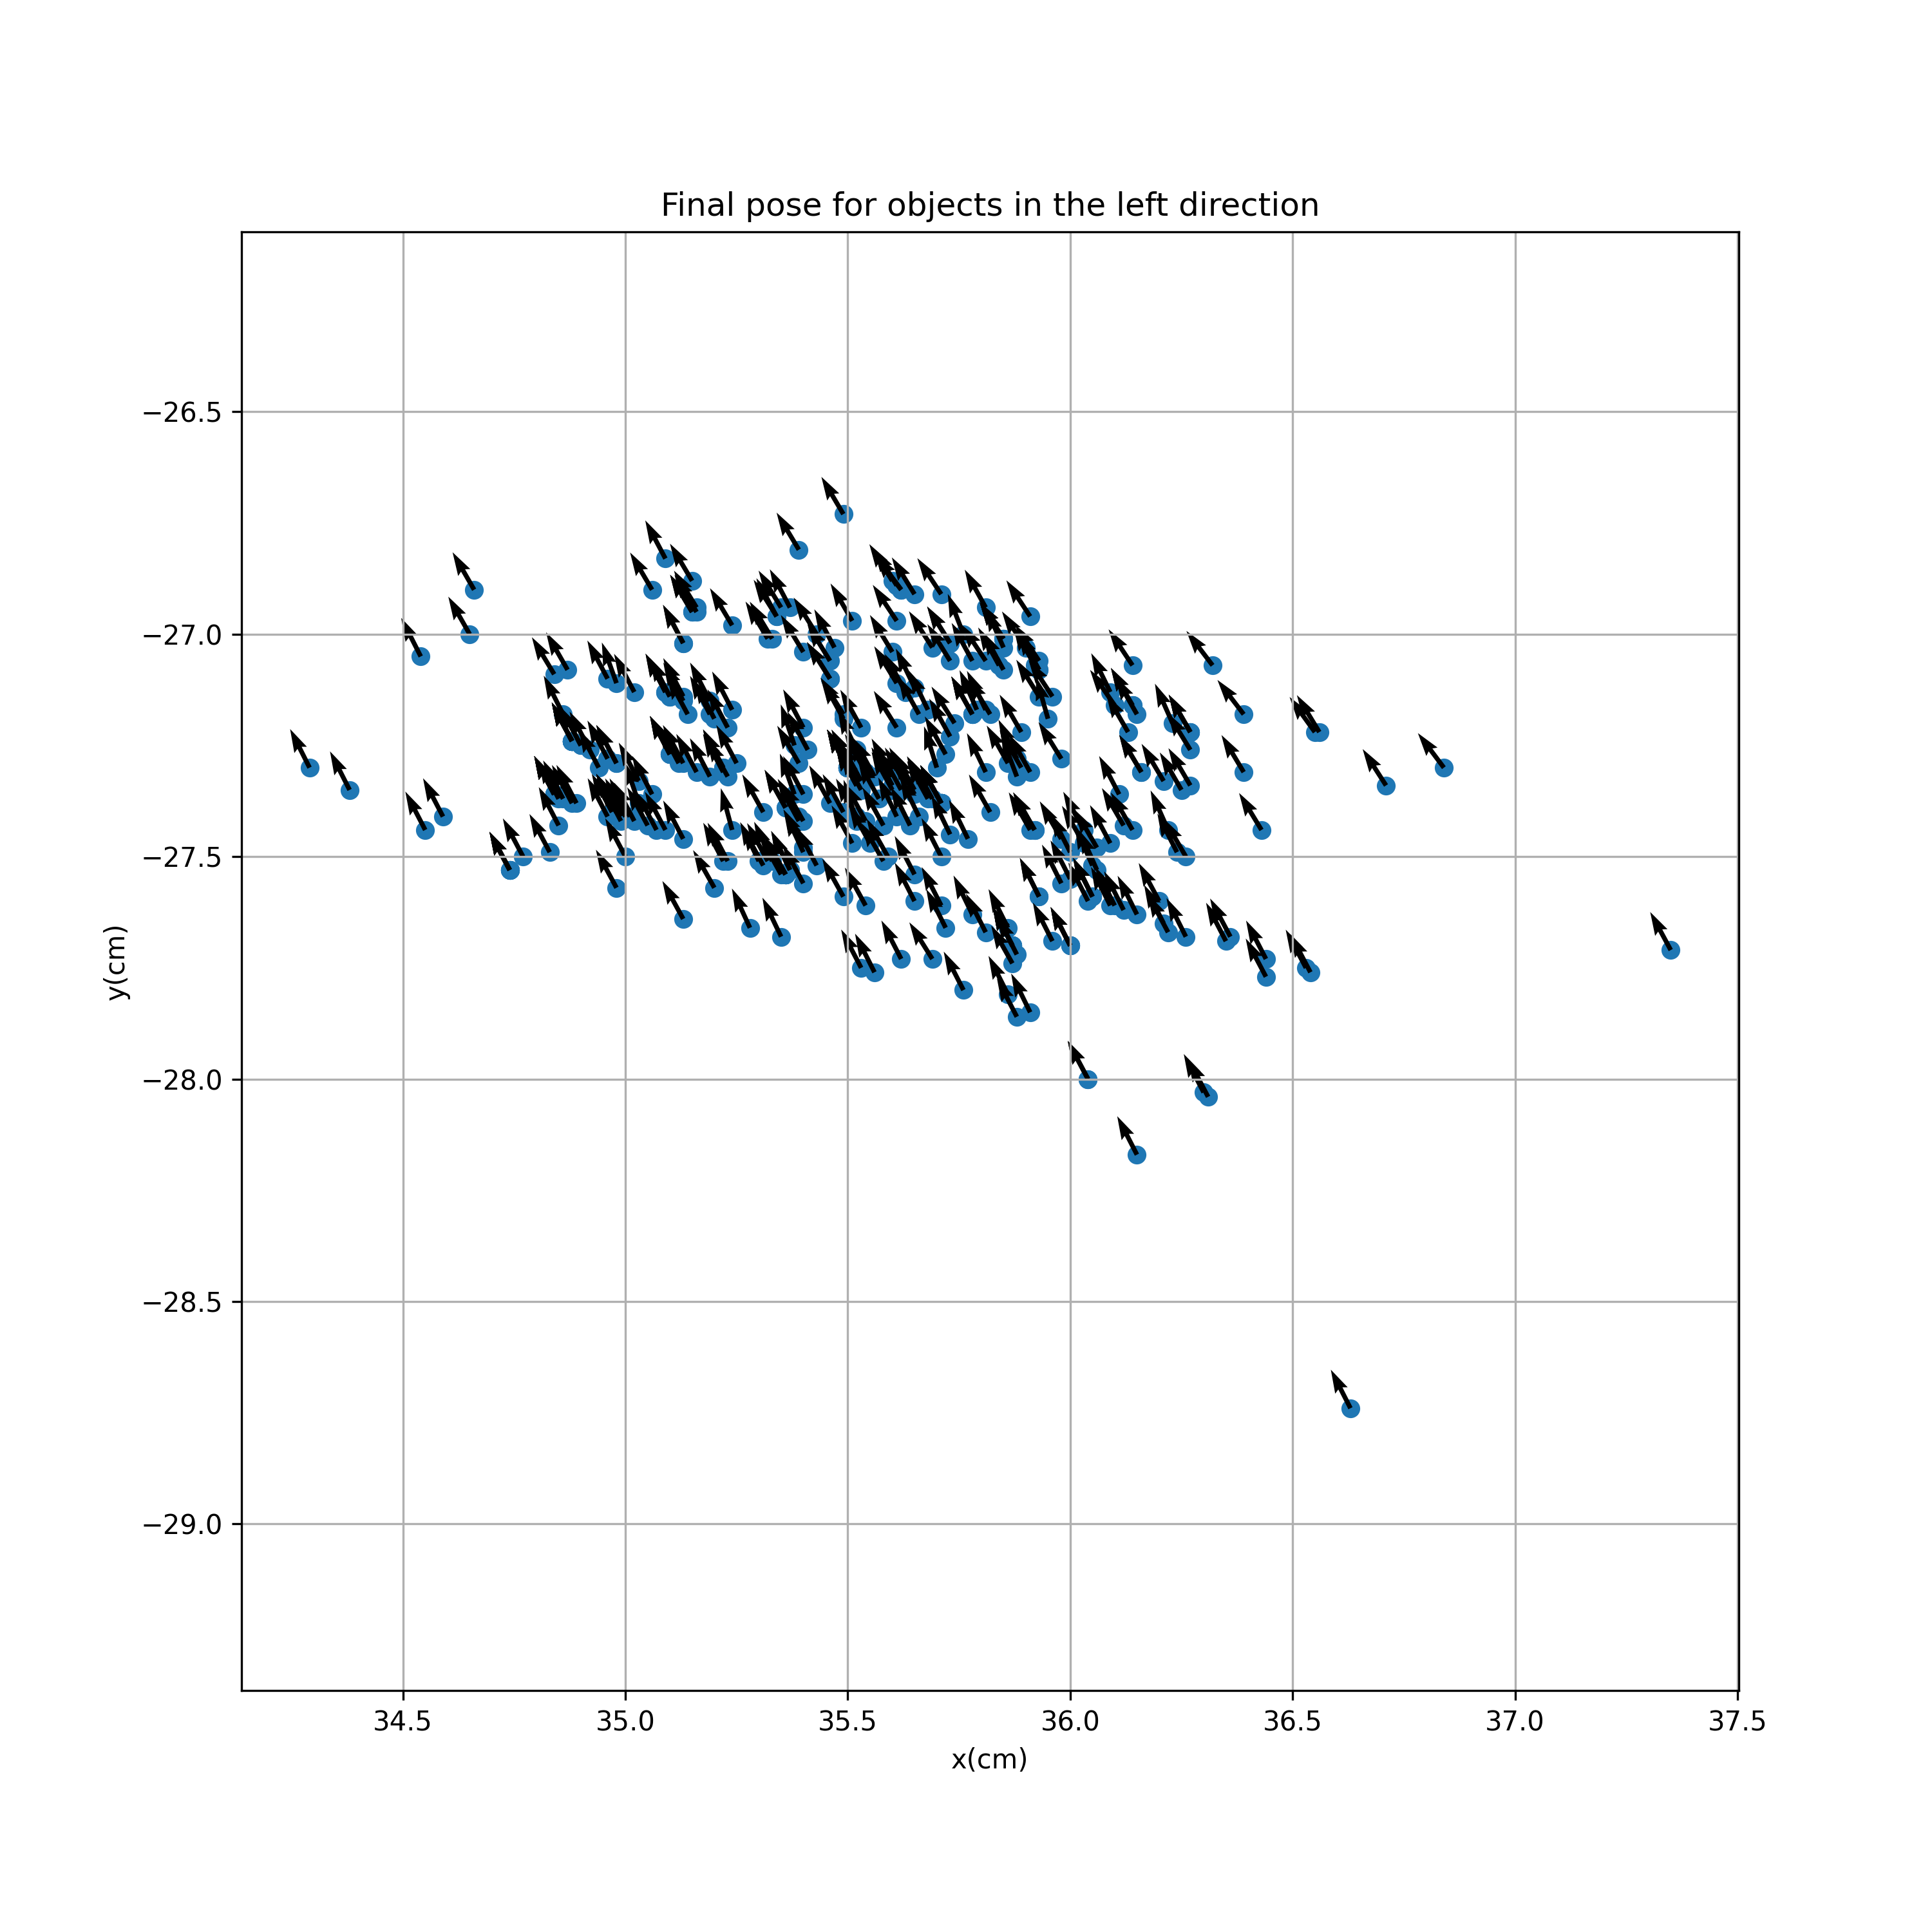
\includegraphics[width=\textwidth]{"images/experiment_5/Final_pose_for_objects_in_the_left_direction.png"}
            \caption{\textcolor{blue}{Left motion before removal of outliers(Object Pose)}}
            \label{fig:exp05-left-end-poses-before}
    \end{figure}
    
    \begin{figure}[H] 
            \centering 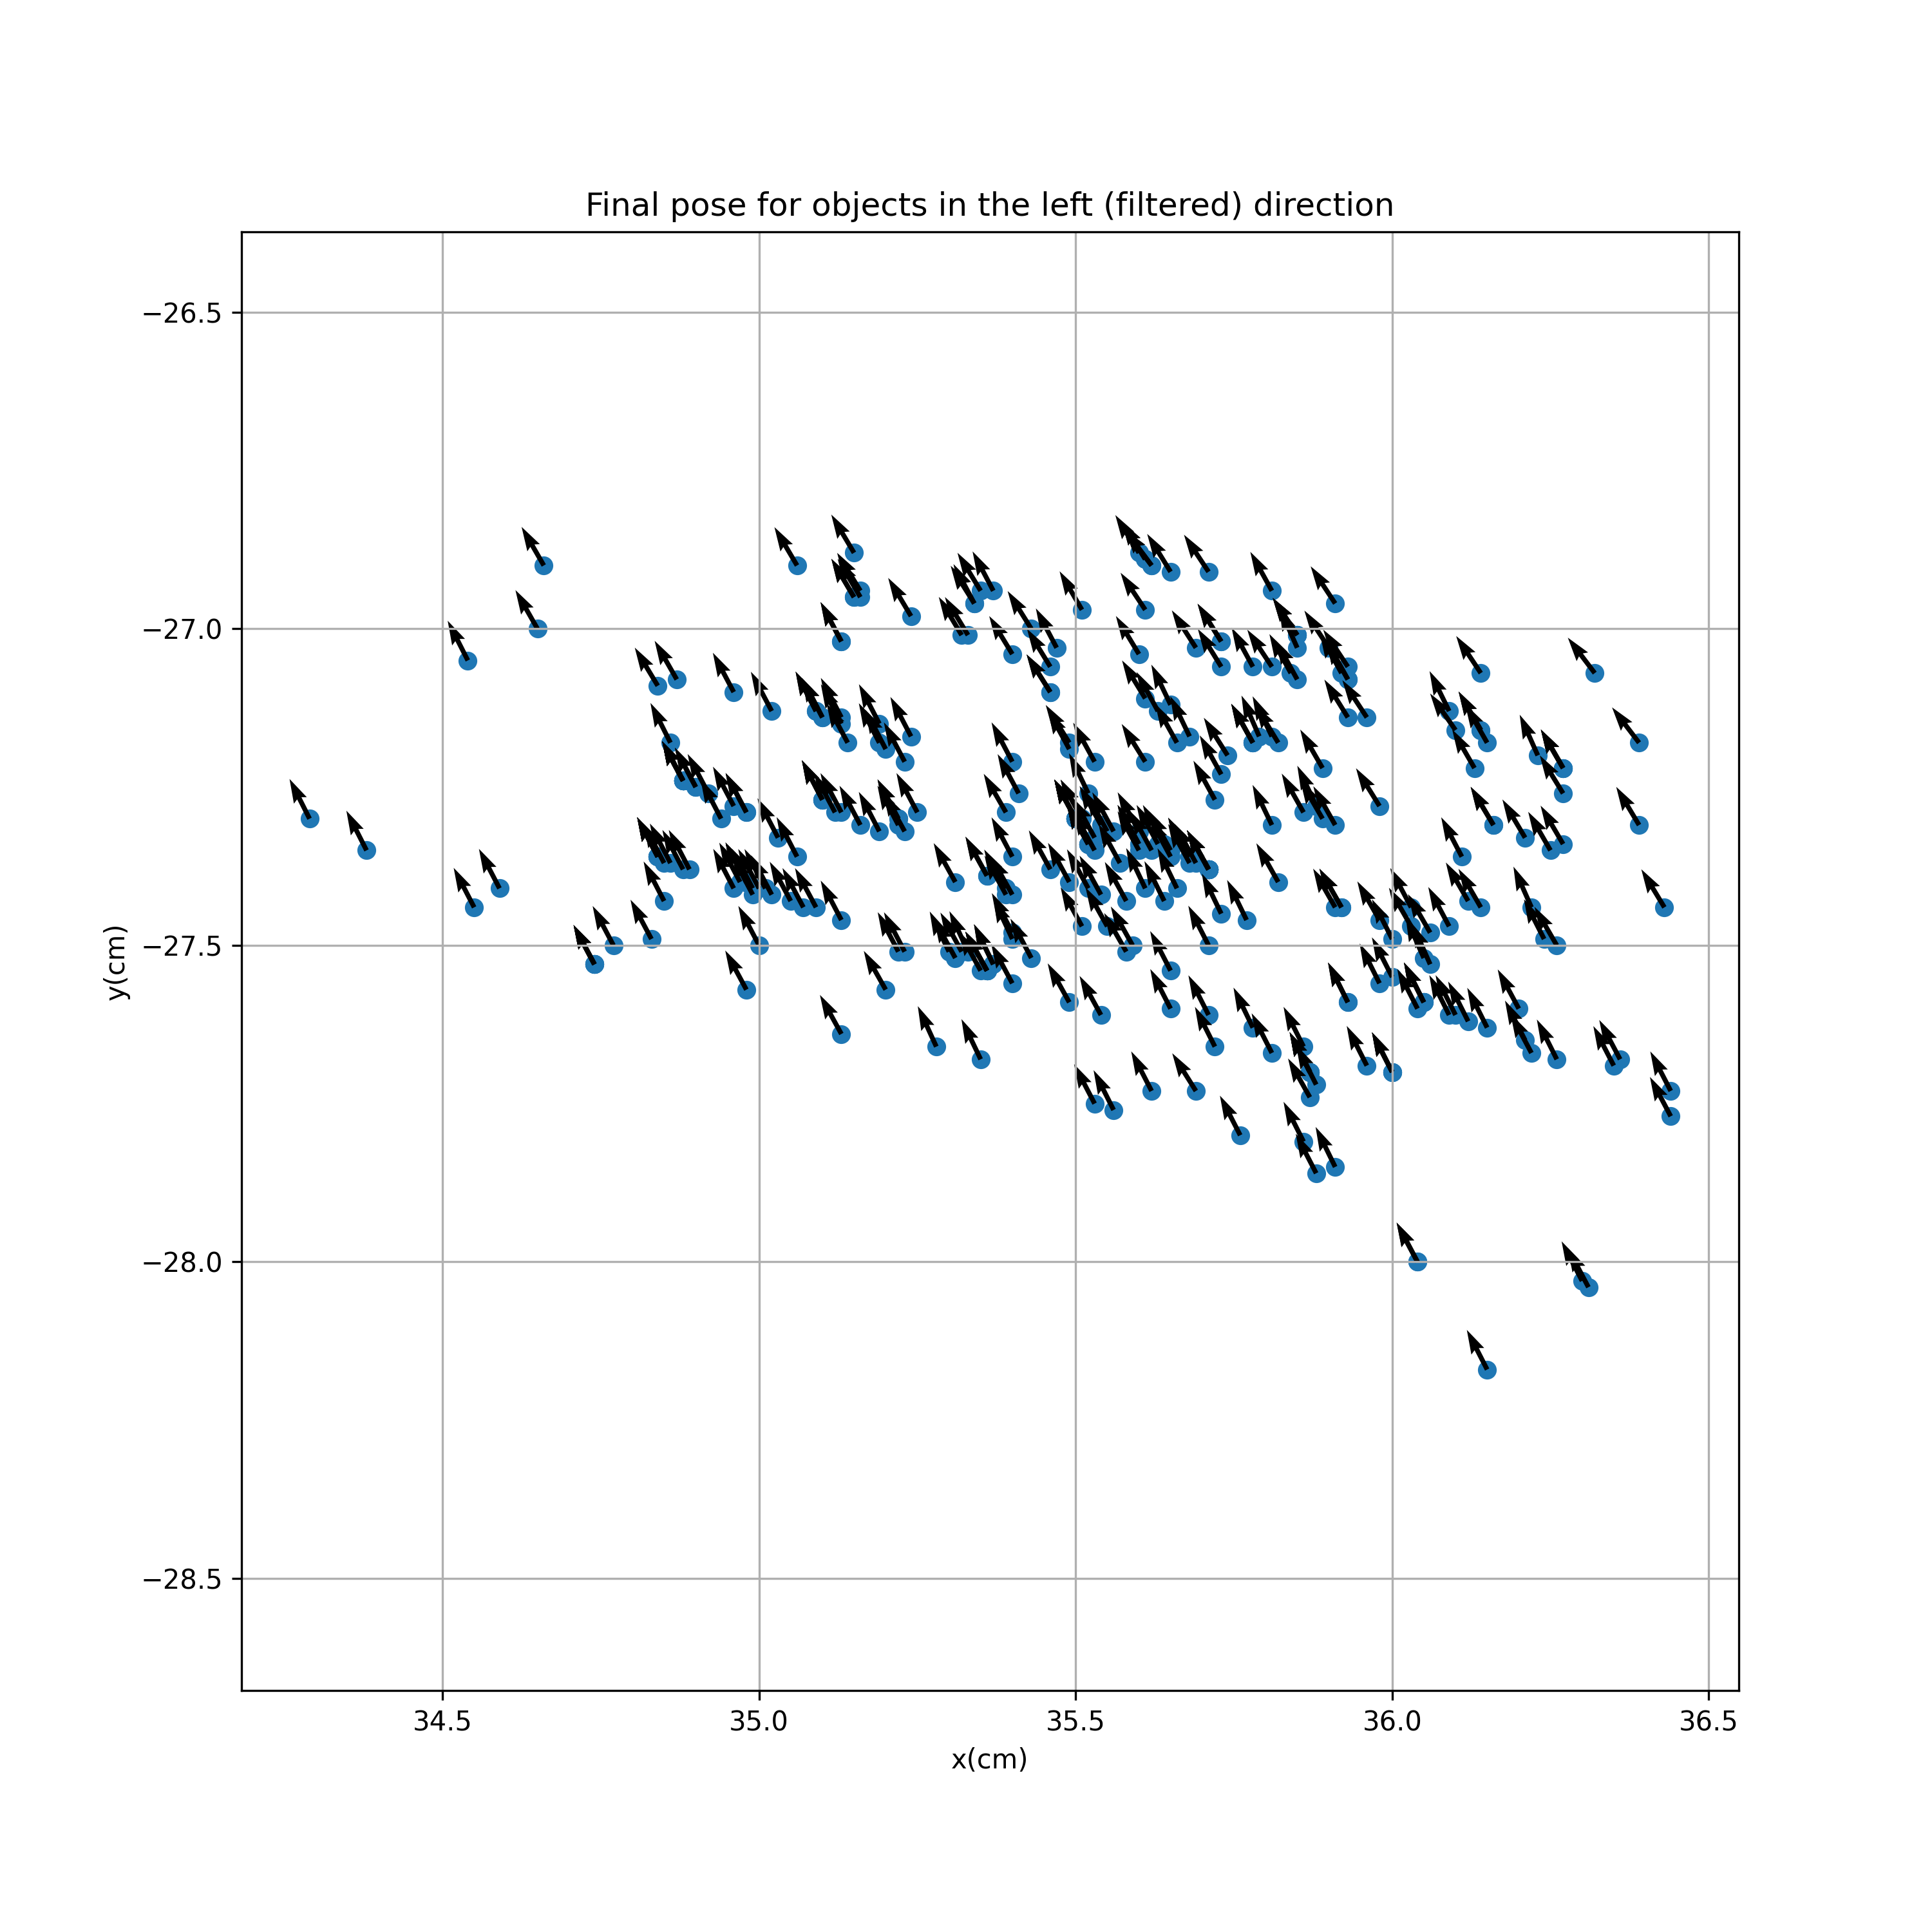
\includegraphics[width=\textwidth]{"images/experiment_5/Final_pose_for_objects_in_the_left (filtered)_direction.png"}
            \caption{\textcolor{blue}{Left motion after removal of outliers(Object Pose)}}
            \label{fig:exp05-left-end-poses-after}
    \end{figure}
    
    % Right motion
    
    \begin{figure}[H] 
            \centering 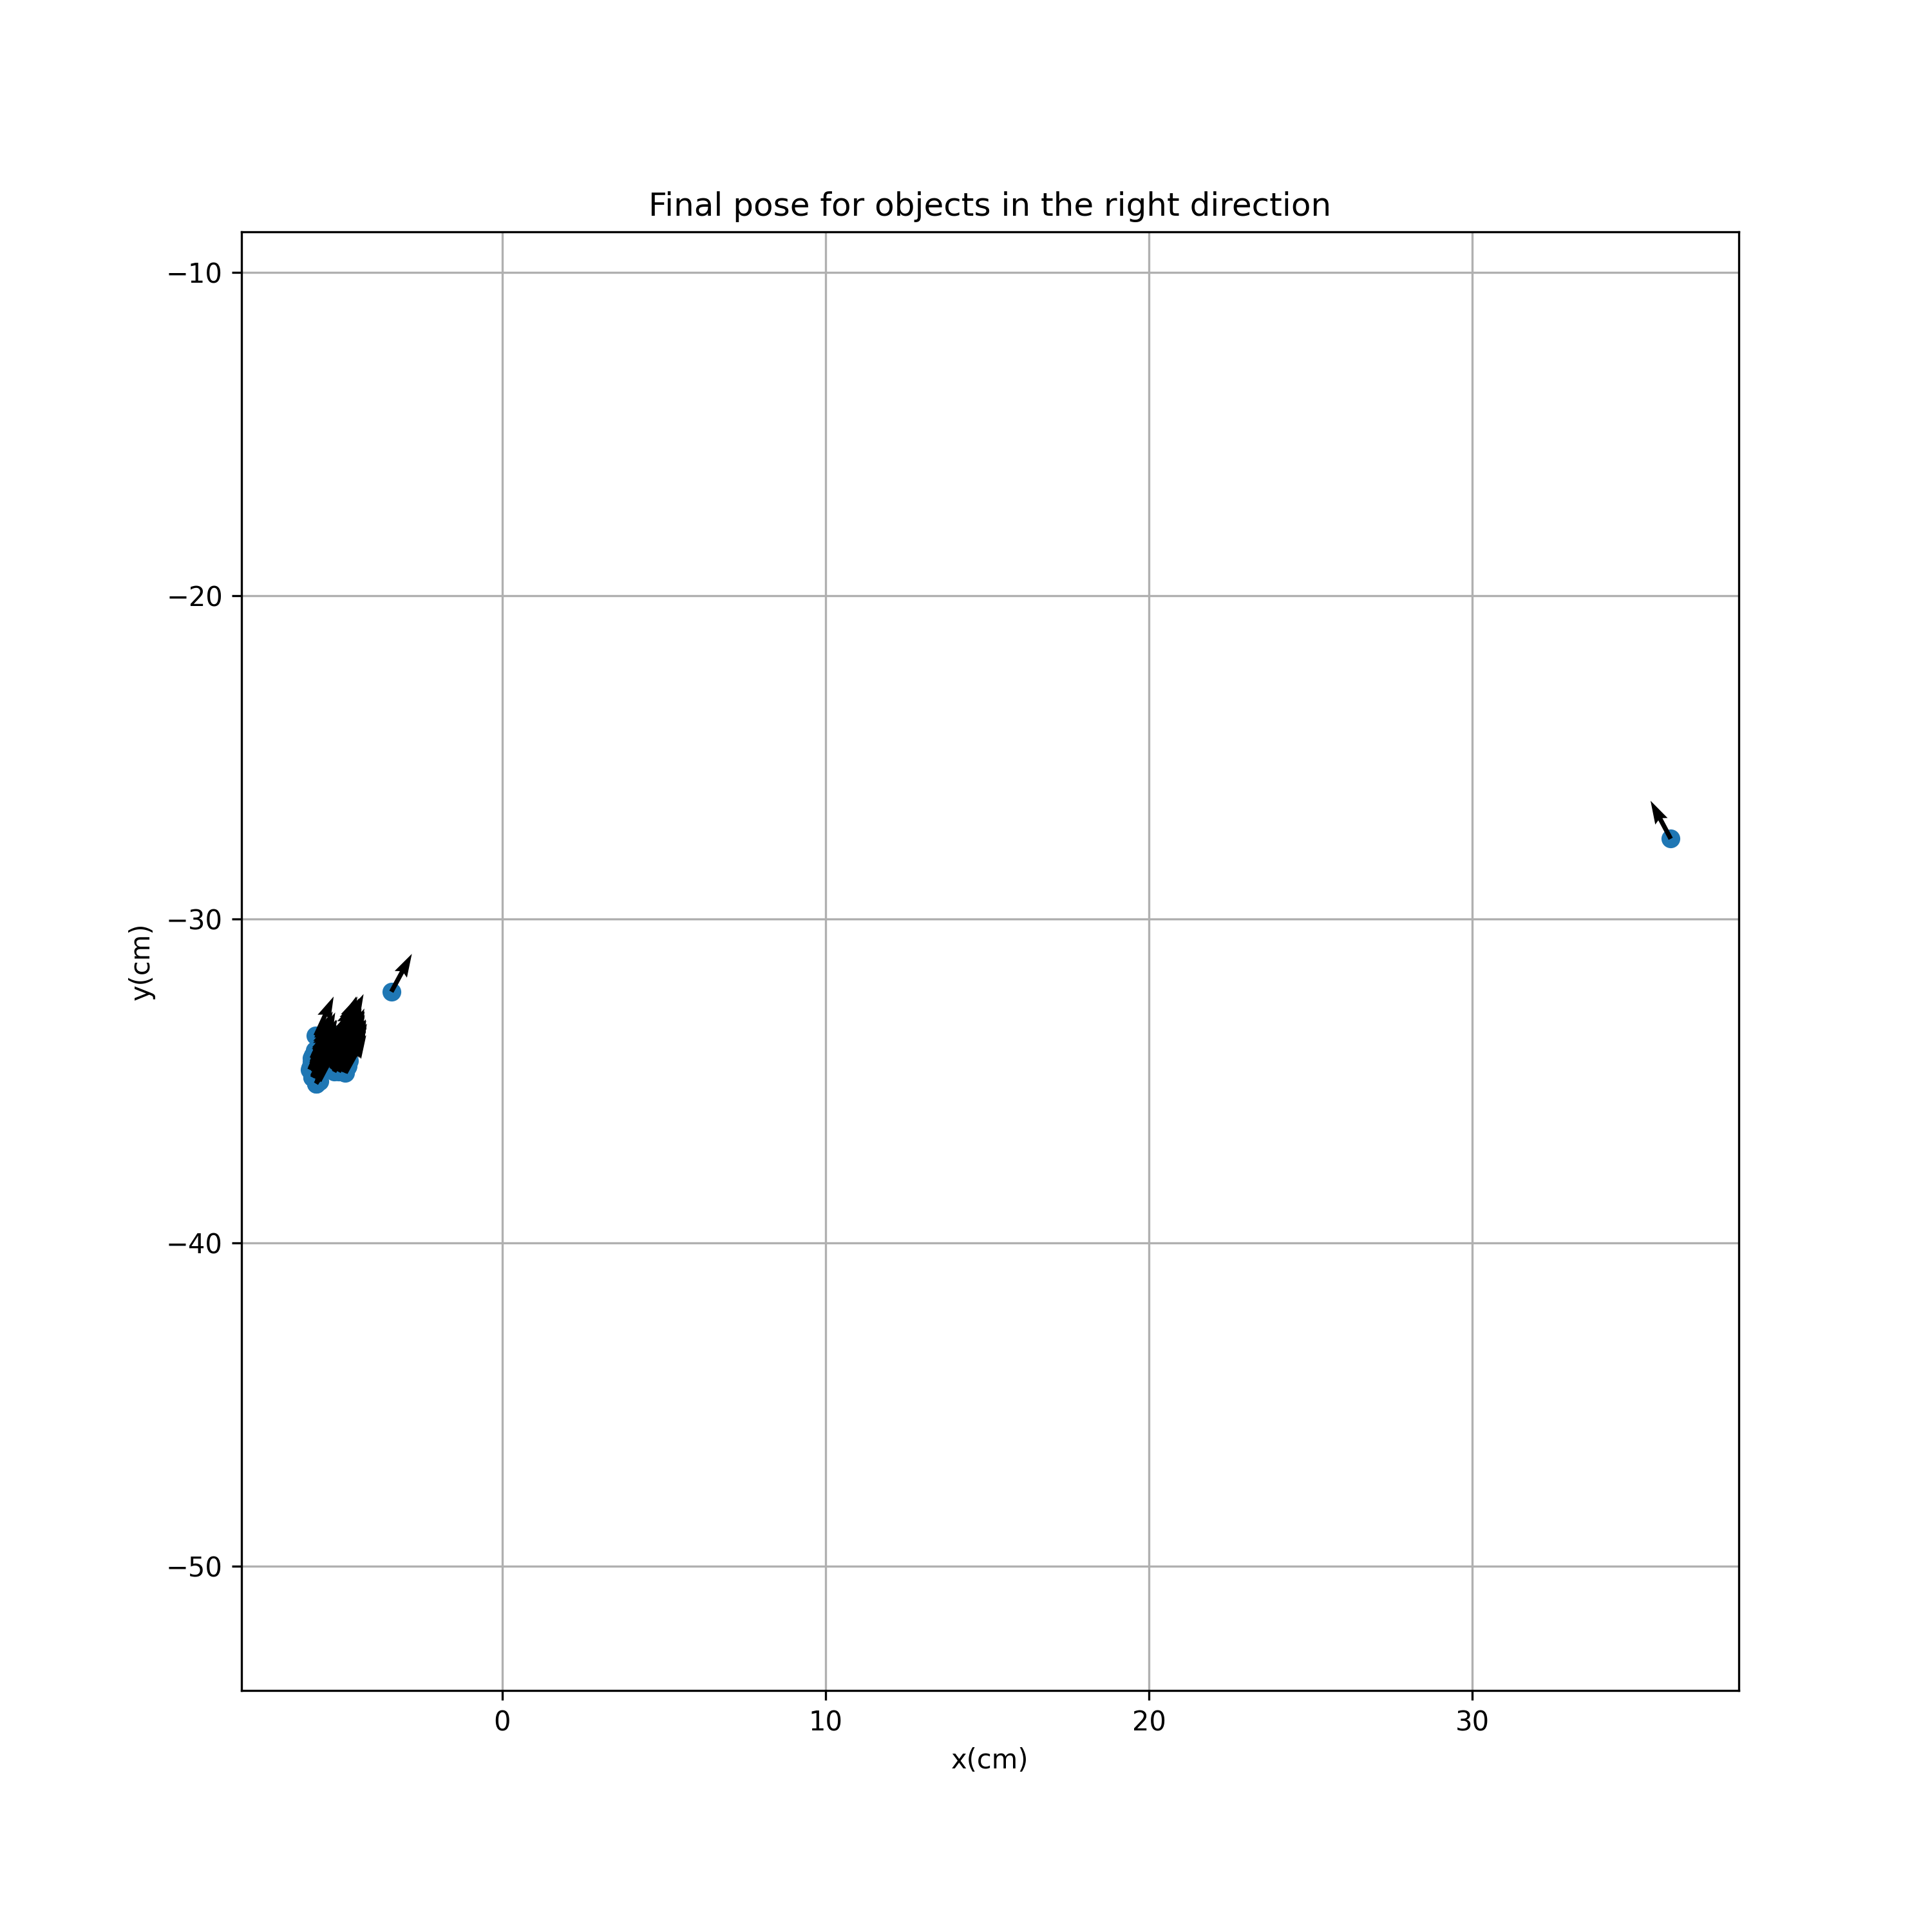
\includegraphics[width=\textwidth]{"images/experiment_5/Final_pose_for_objects_in_the_right_direction.png"}
            \caption{\textcolor{blue}{Right motion before removal of outliers(Object Pose)}}
            \label{fig:exp05-right-end-poses-before}
    \end{figure}
    
    \begin{figure}[H] 
            \centering 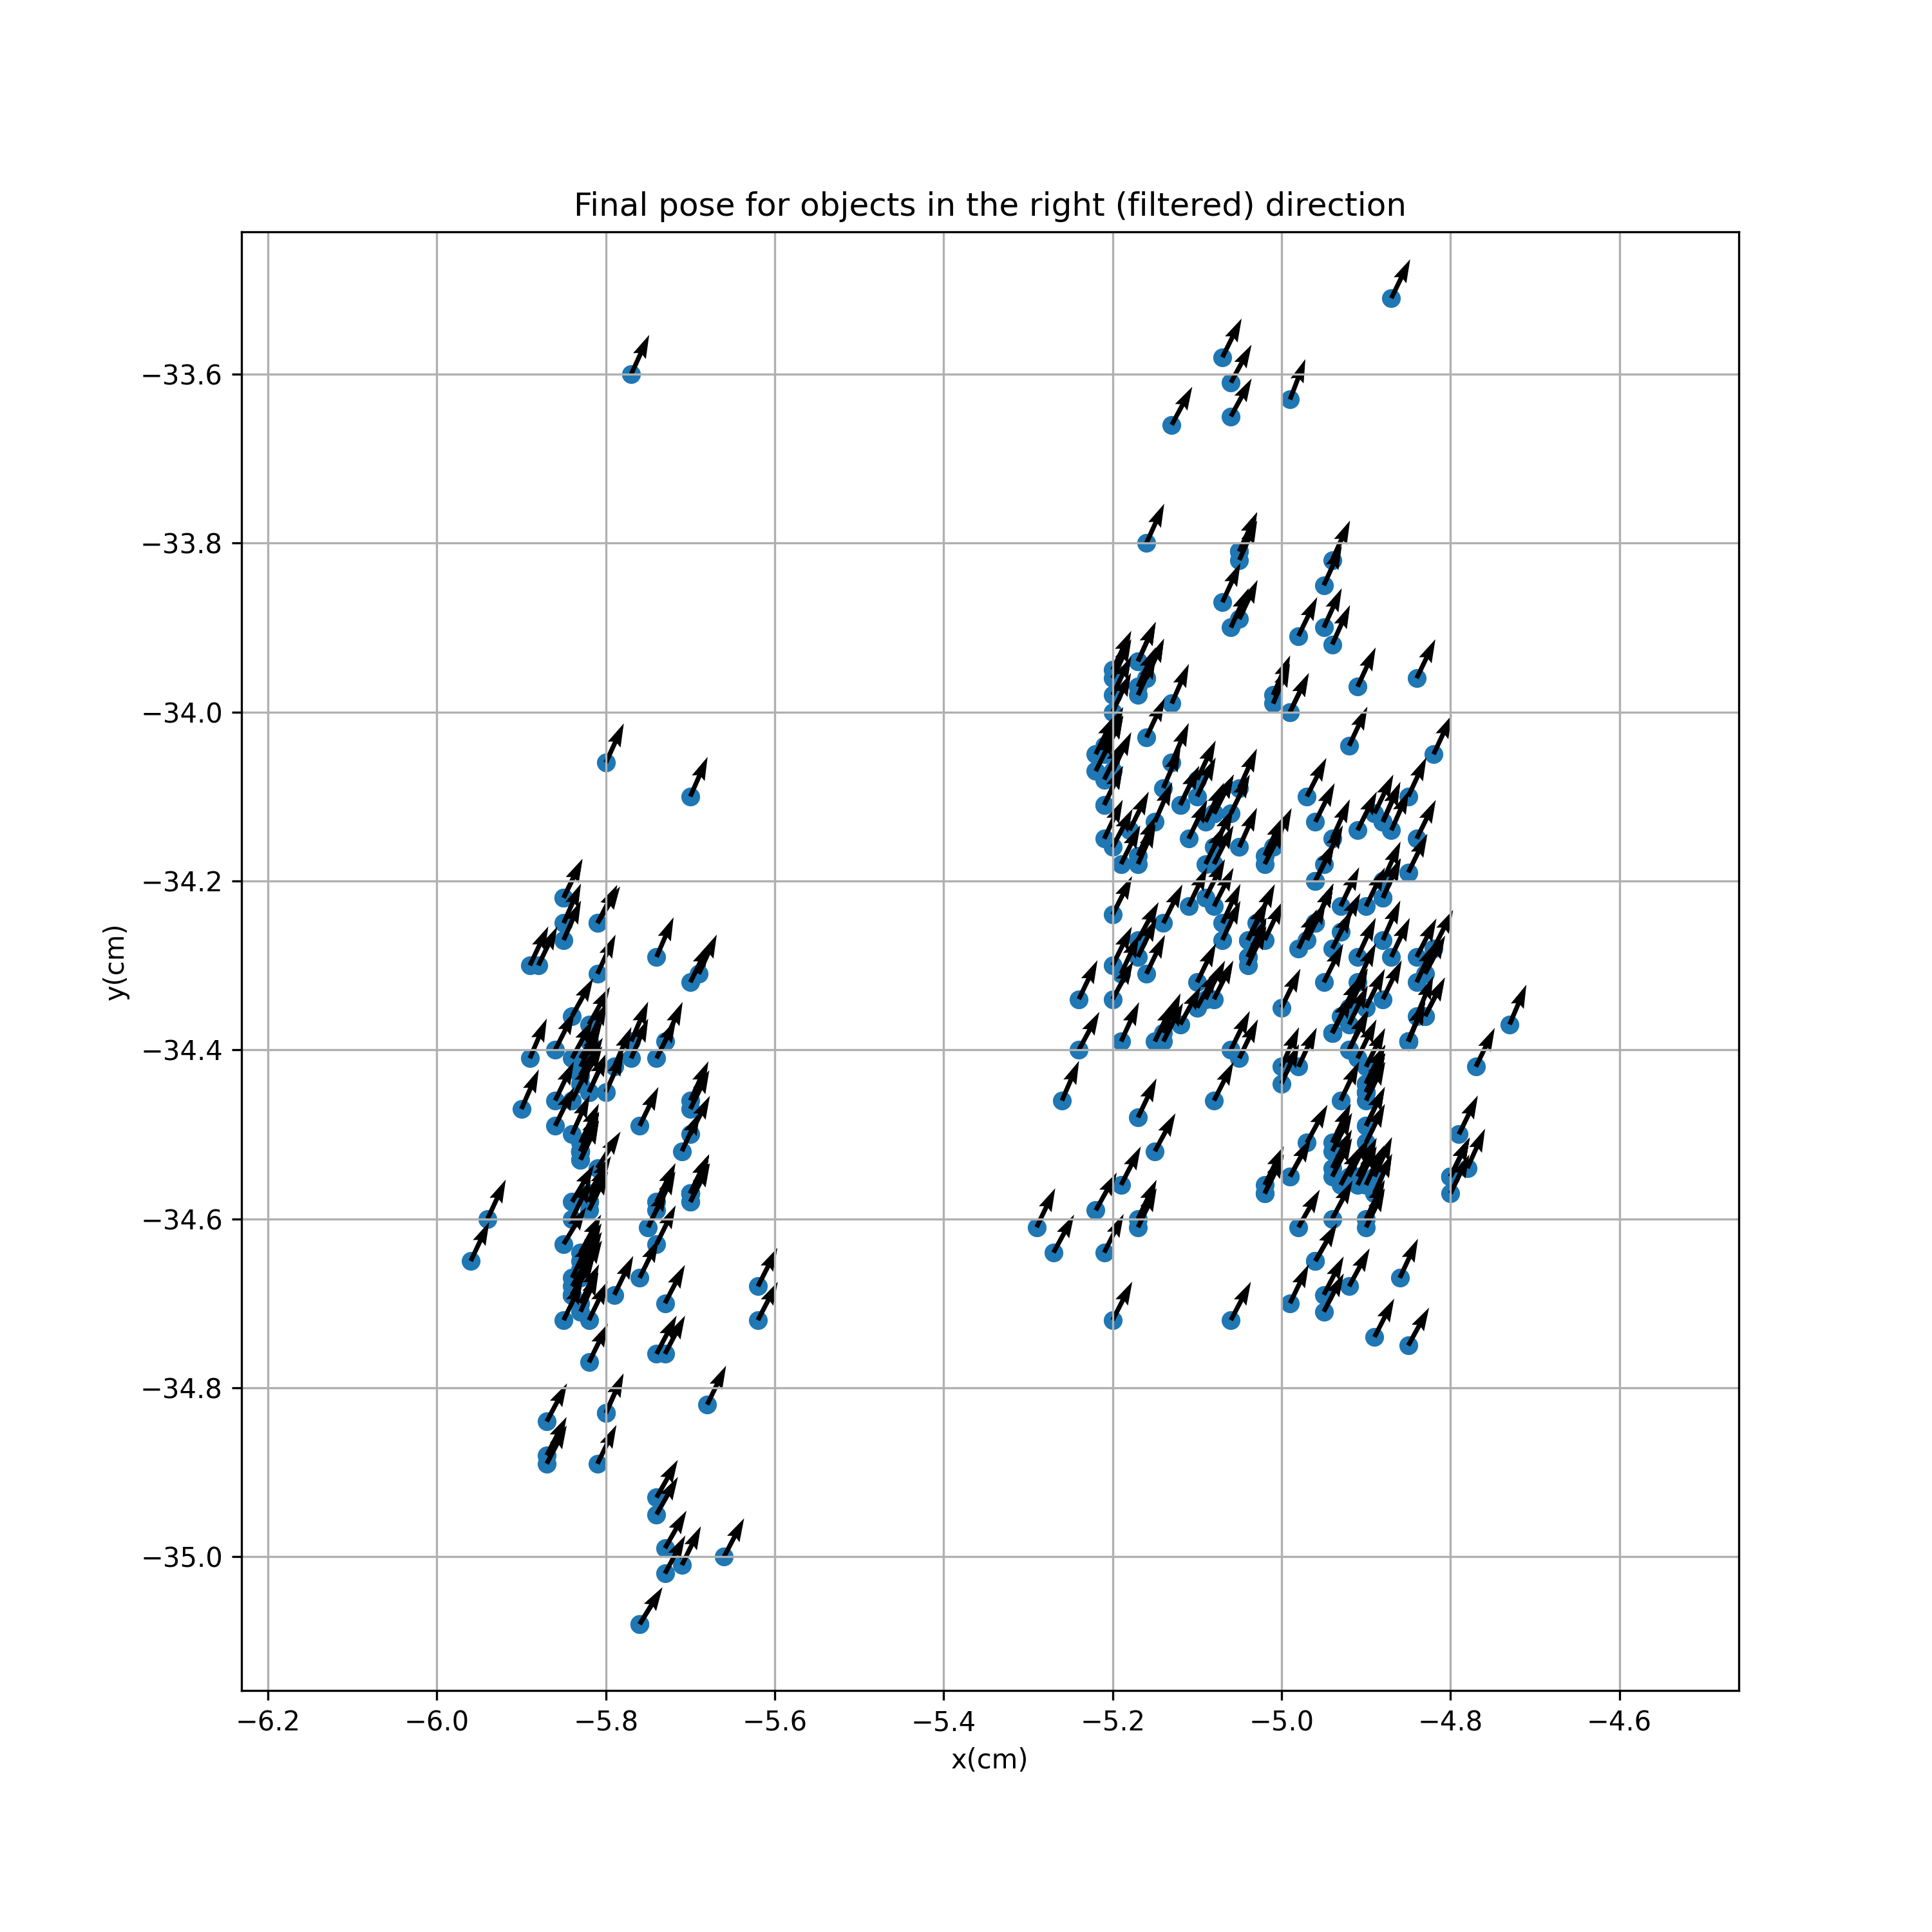
\includegraphics[width=\textwidth]{"images/experiment_5/Final_pose_for_objects_in_the_right (filtered)_direction.png"}
            \caption{\textcolor{blue}{Right motion after removal of outliers(Object Pose)}}
            \label{fig:exp05-right-end-poses-after}
    \end{figure}
    
    
    
        \begin{figure}[H] 
            \centering 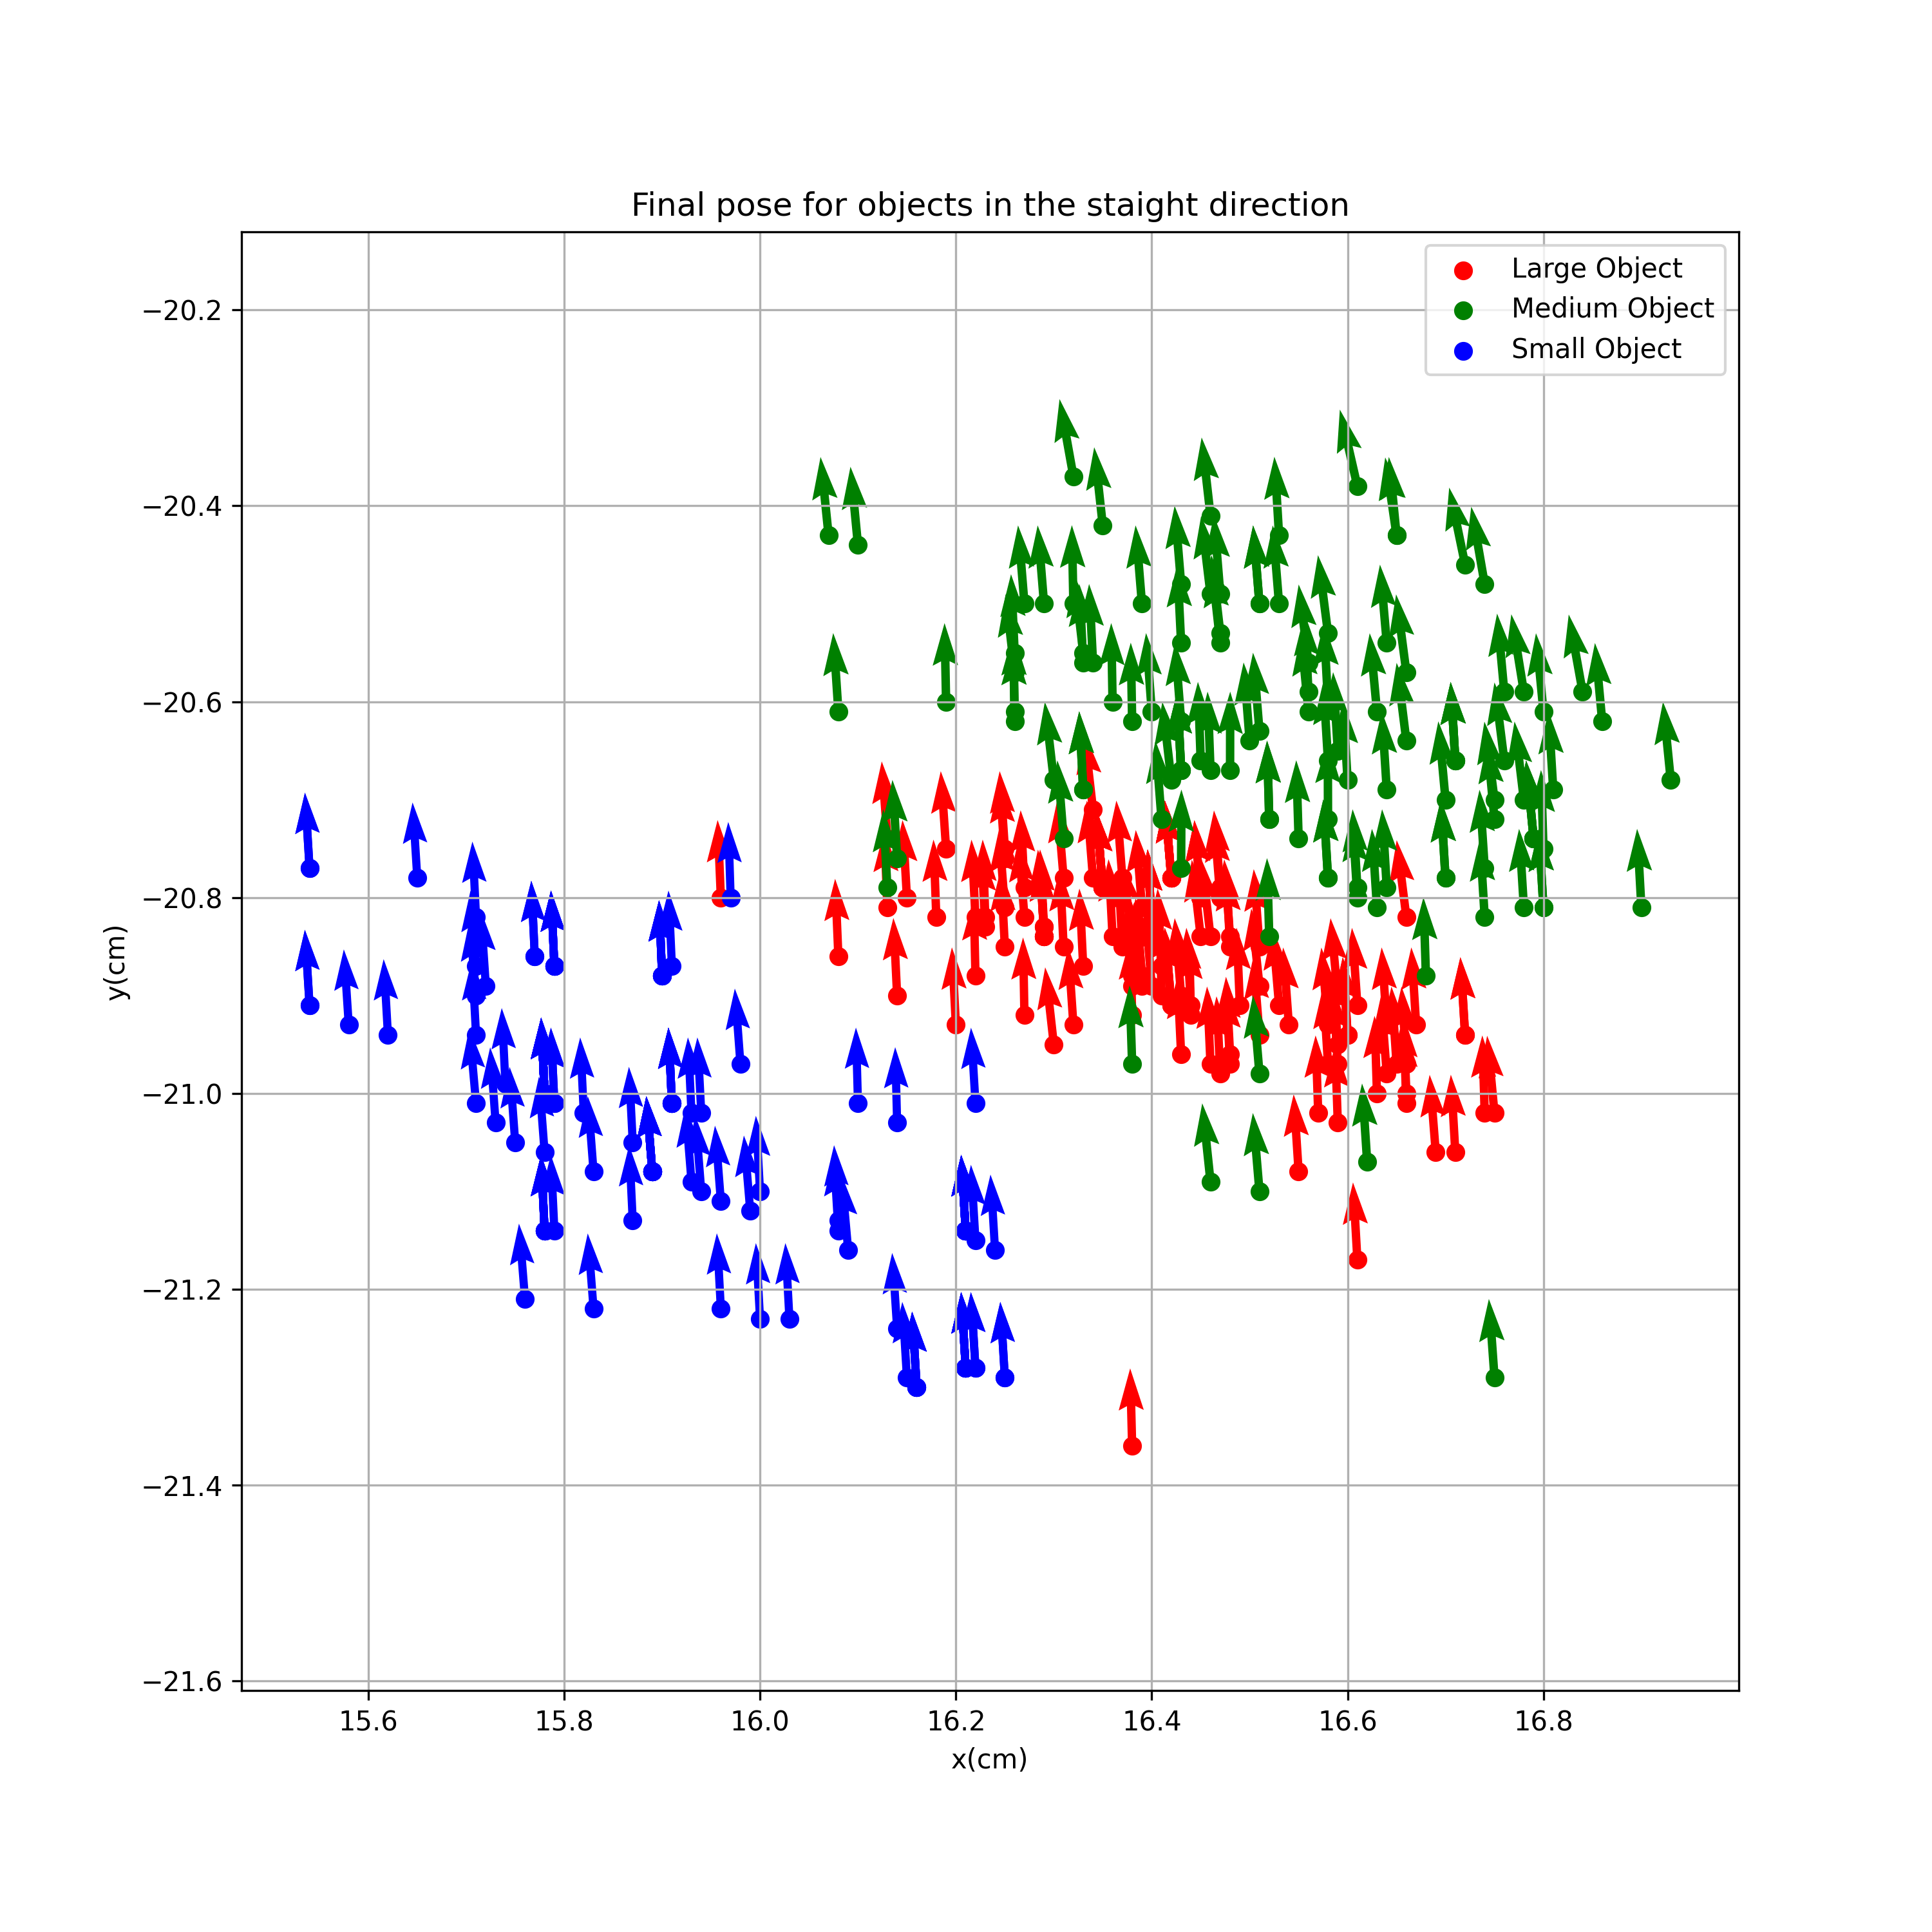
\includegraphics[width=\textwidth]{"images/experiment_5/Final_pose_for_objects_of_different_size_striaght.png"}
            \caption{\textcolor{blue}{Straight motion object pose of all sizes}}
            \label{fig:exp05-straight-end-poses-all-size}
    \end{figure}
    
    
    
        \begin{figure}[H] 
            \centering 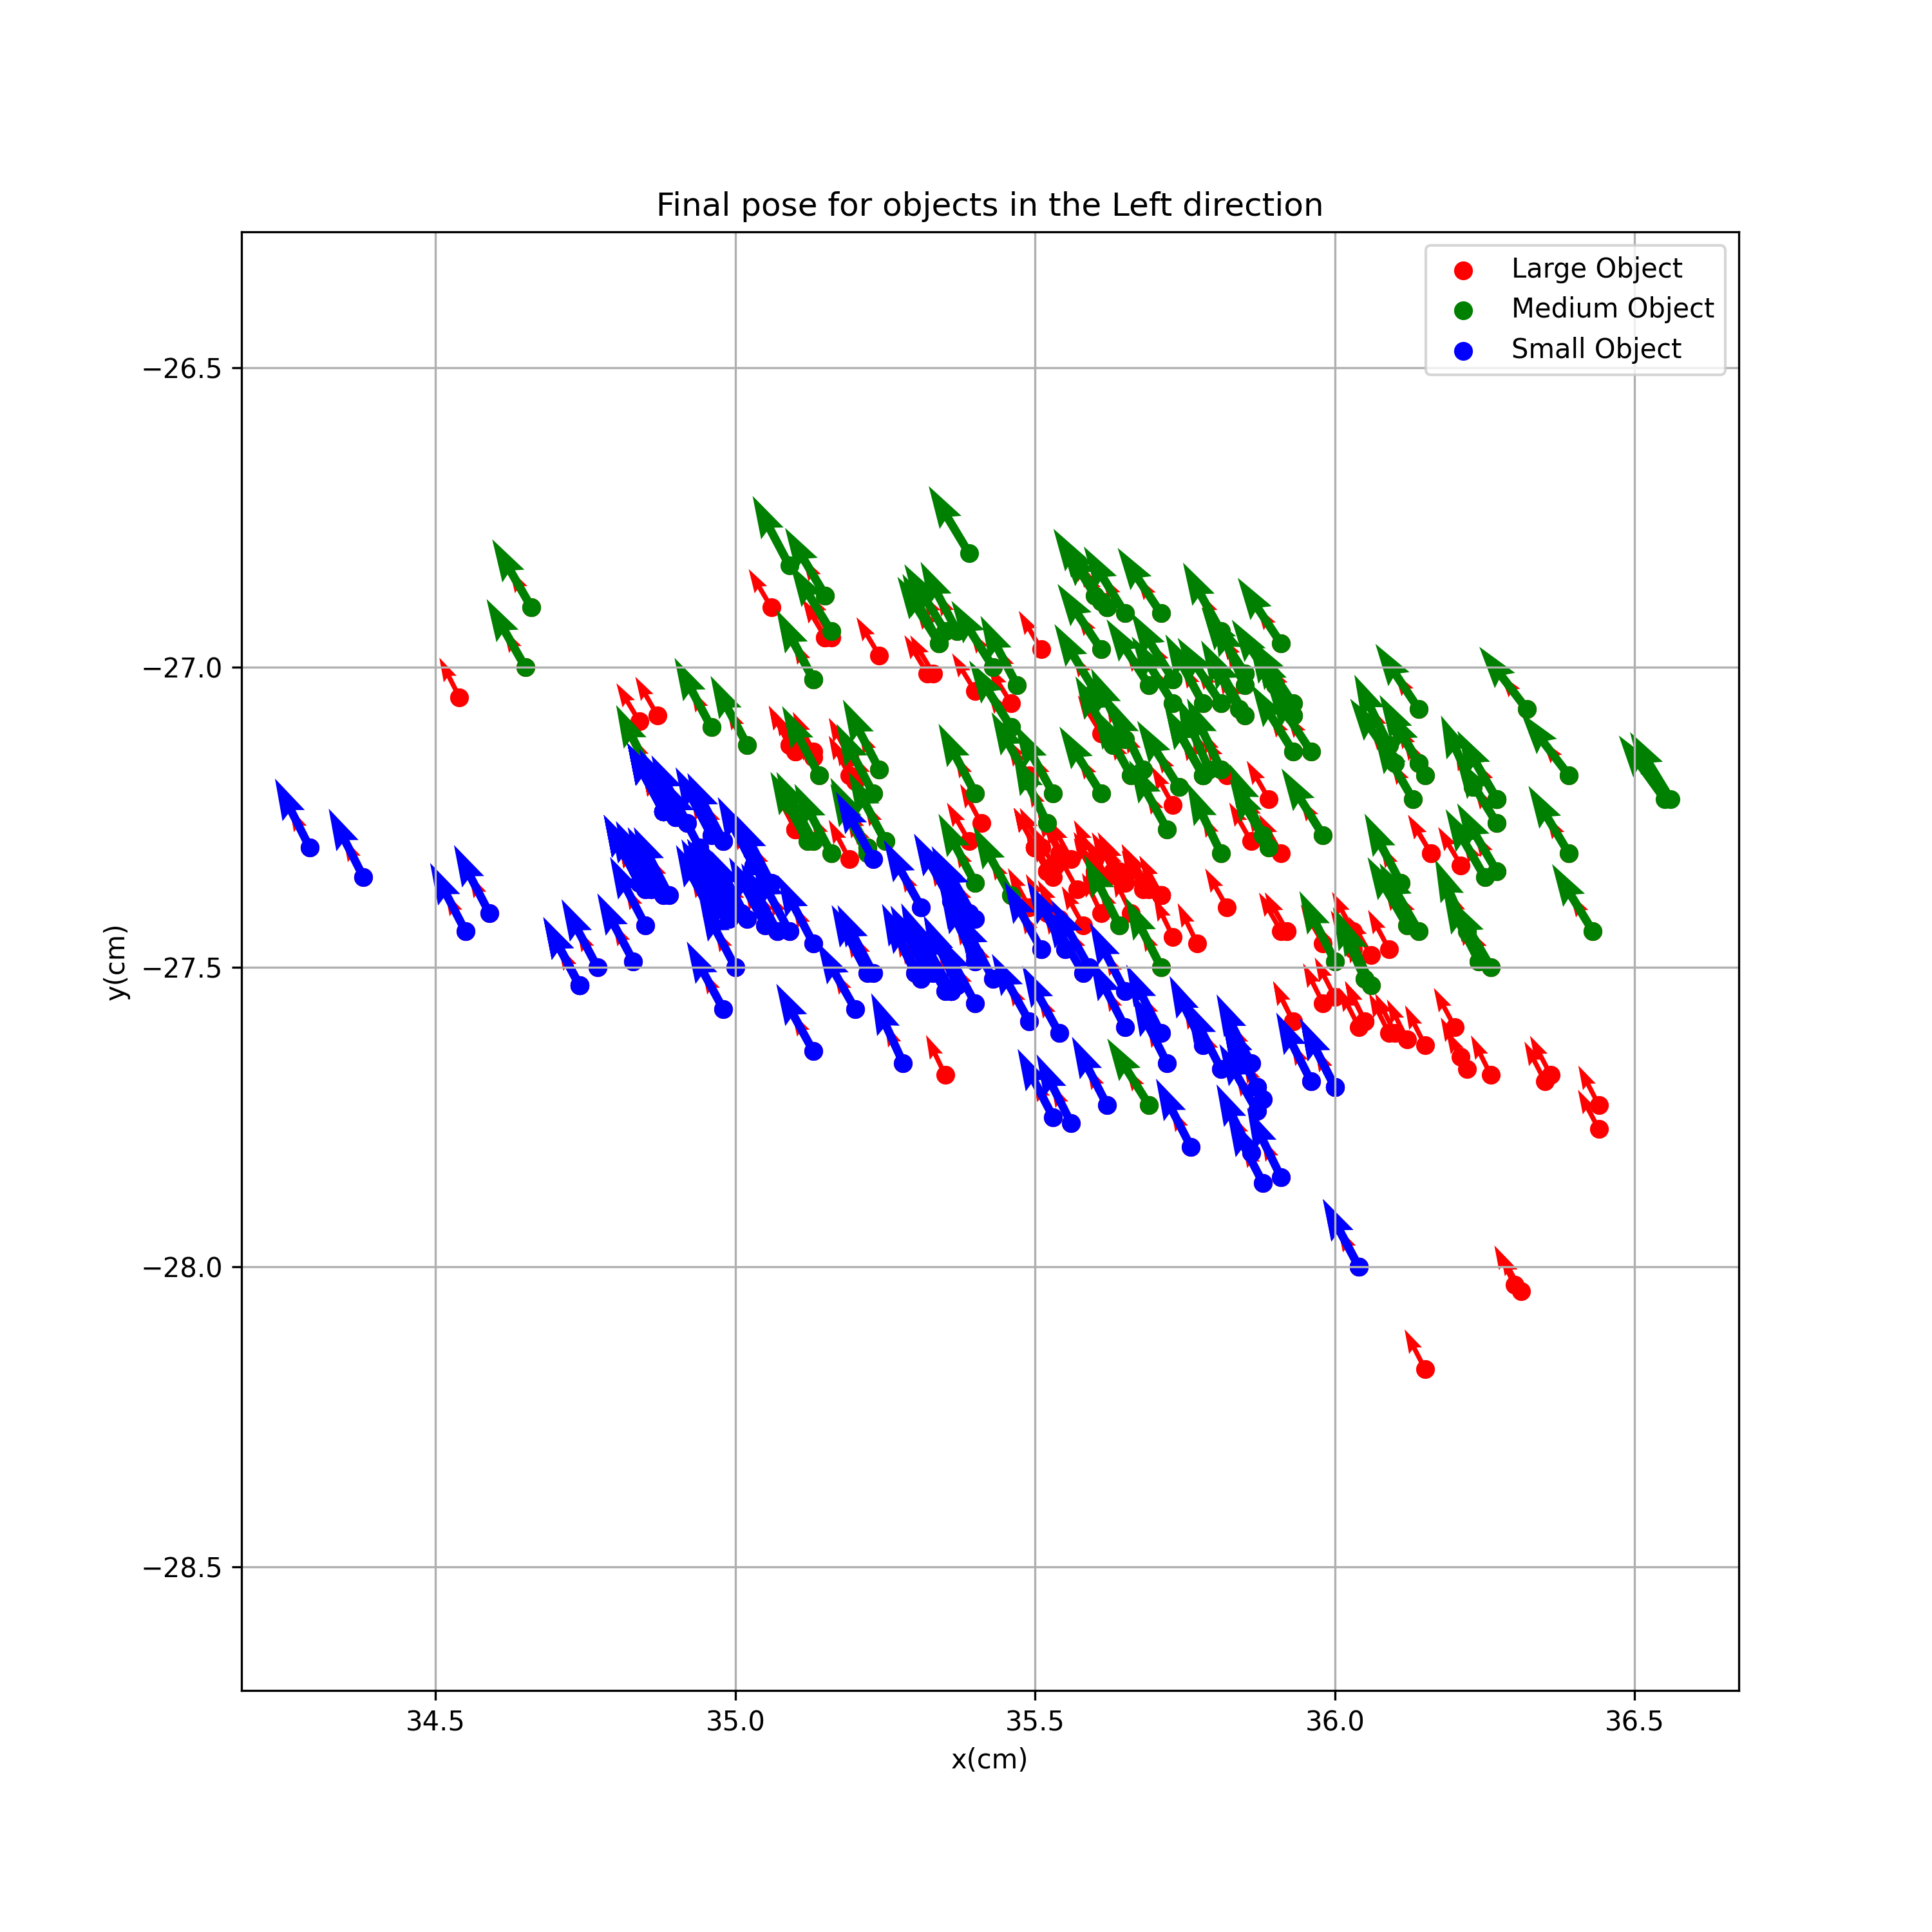
\includegraphics[width=\textwidth]{"images/experiment_5/Final_pose_for_objects_of_different_size_left.png"}
            \caption{\textcolor{blue}{Left motion object pose of all sizes}}
            \label{fig:exp05-left-end-poses-all-size}
    \end{figure}
    
    
        \begin{figure}[H] 
            \centering 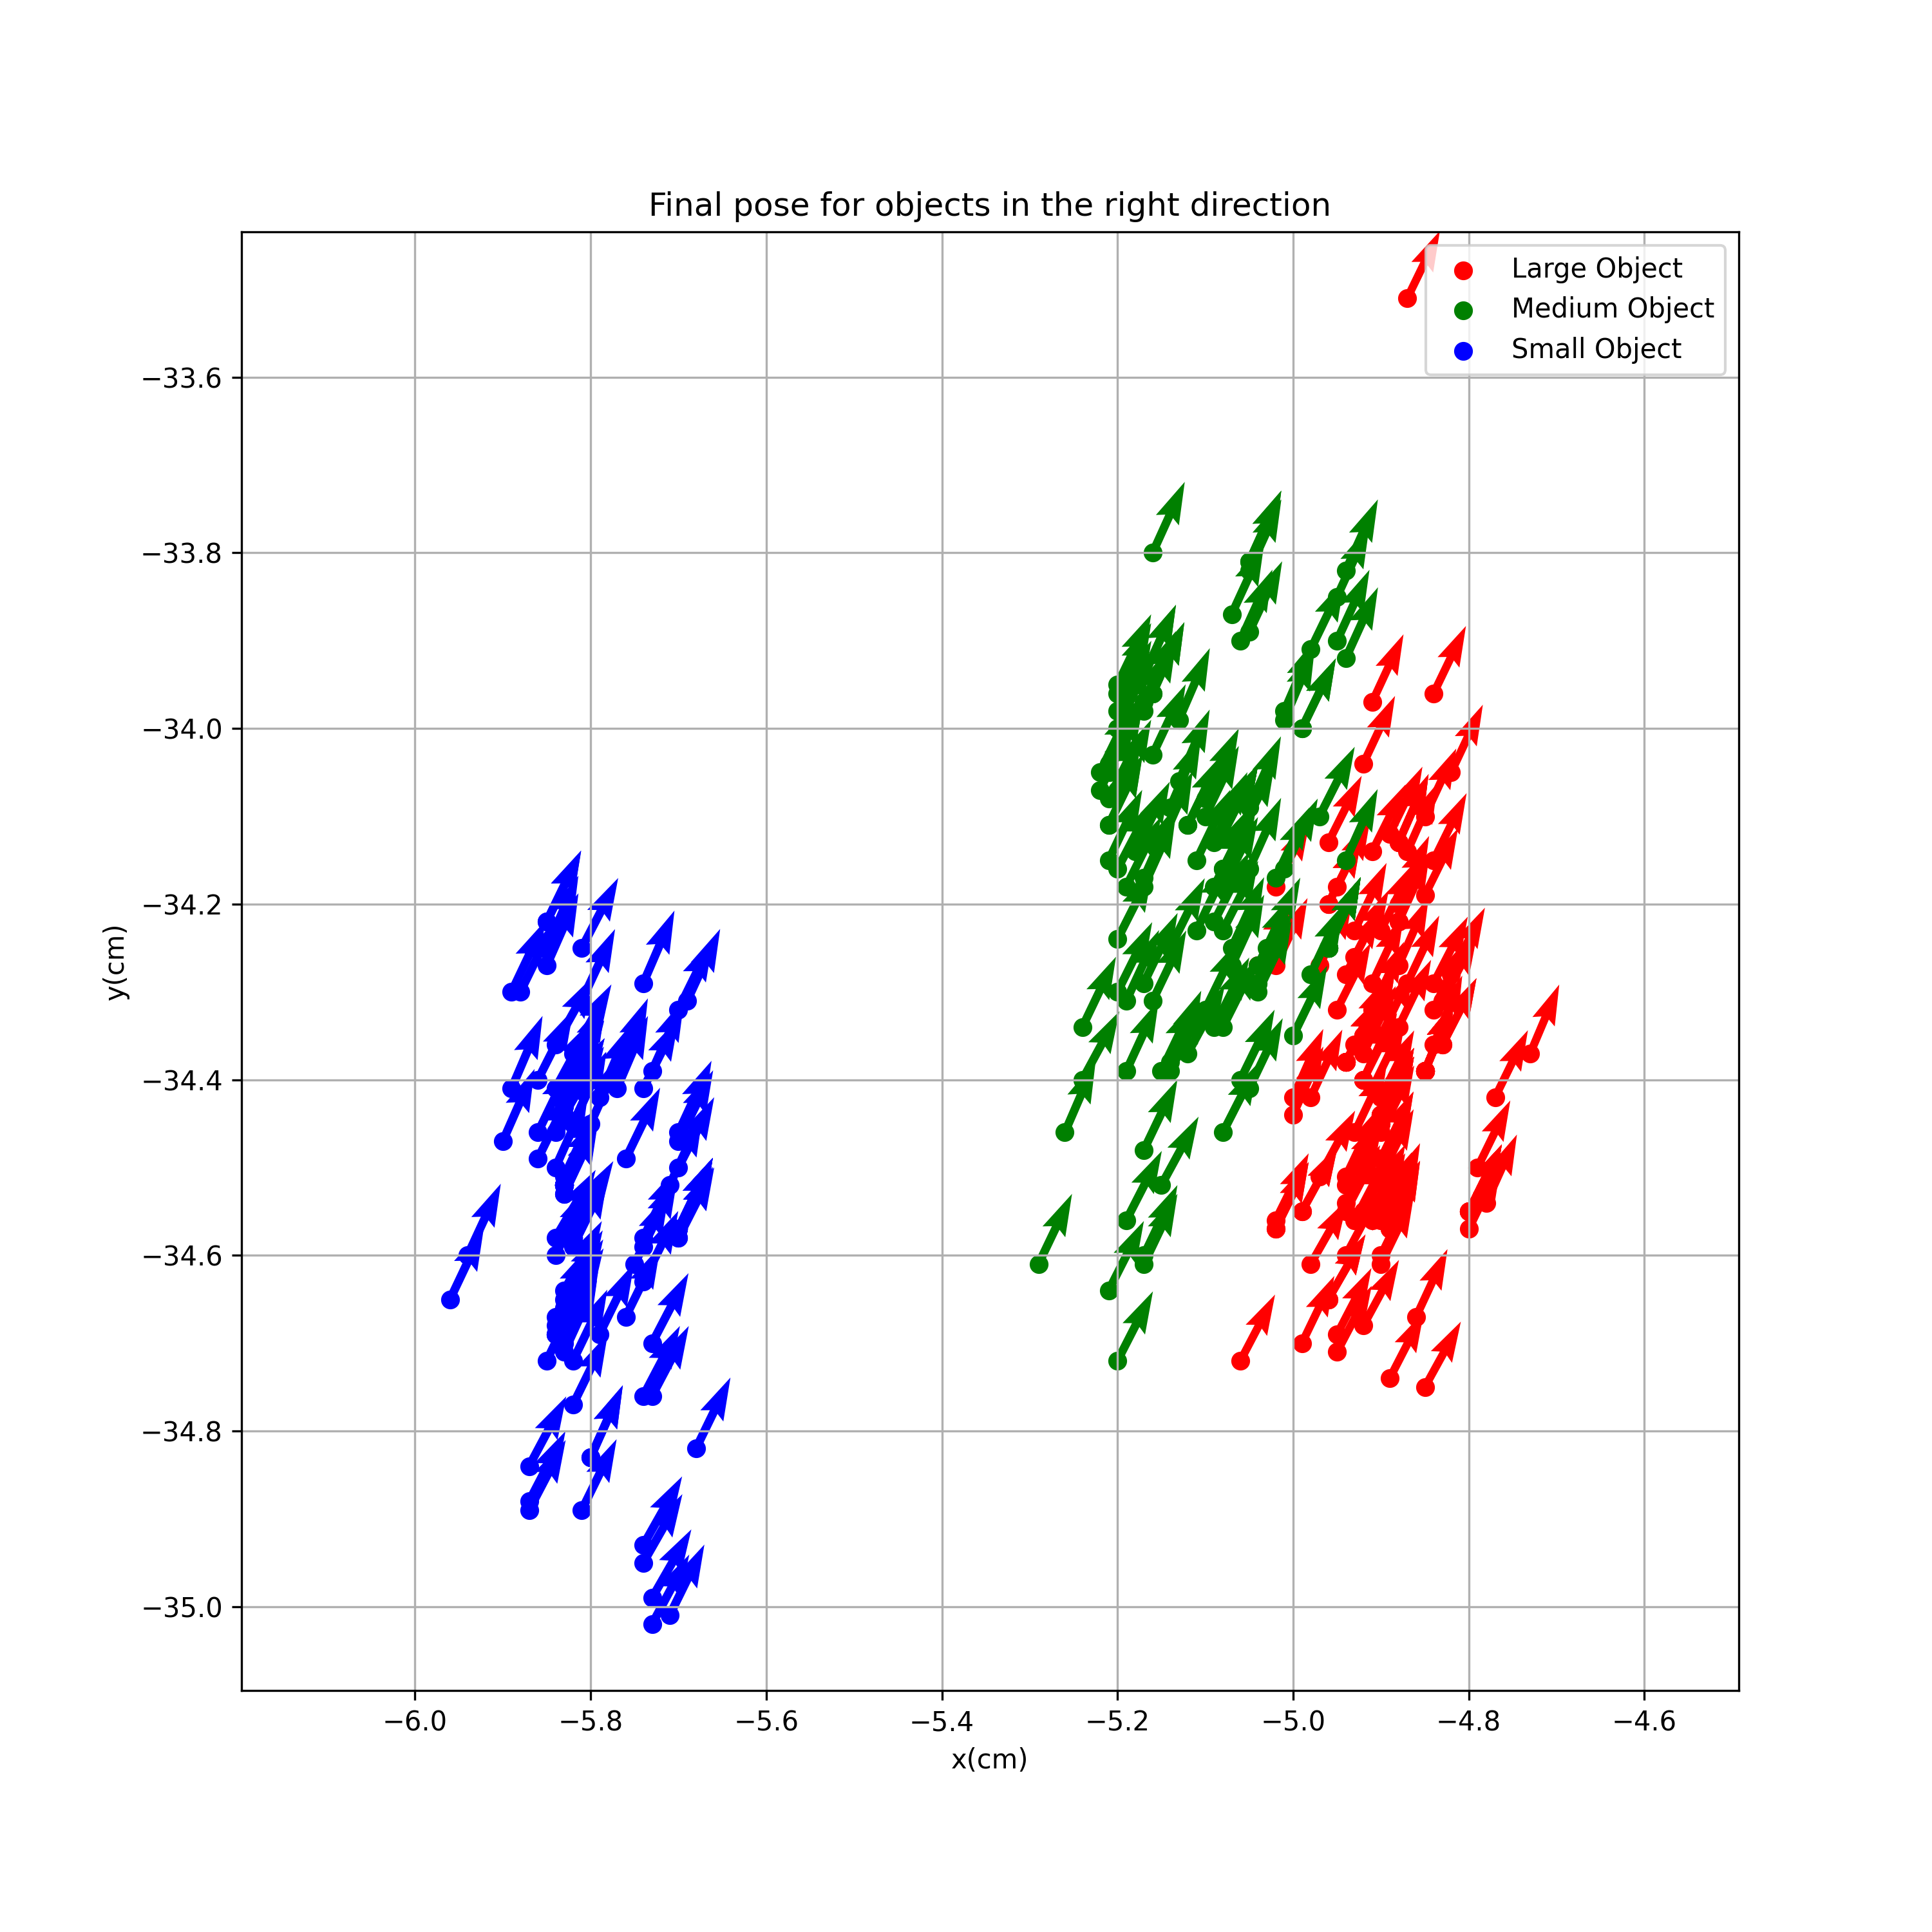
\includegraphics[width=\textwidth]{"images/experiment_5/Final_pose_for_objects_of_different_size_right.png"}
            \caption{\textcolor{blue}{Right motion object pose of all sizes}}
            \label{fig:exp05-right-end-all-size}
    \end{figure}
    
    % Trajecory
    
    \begin{figure}[H] 
            \centering 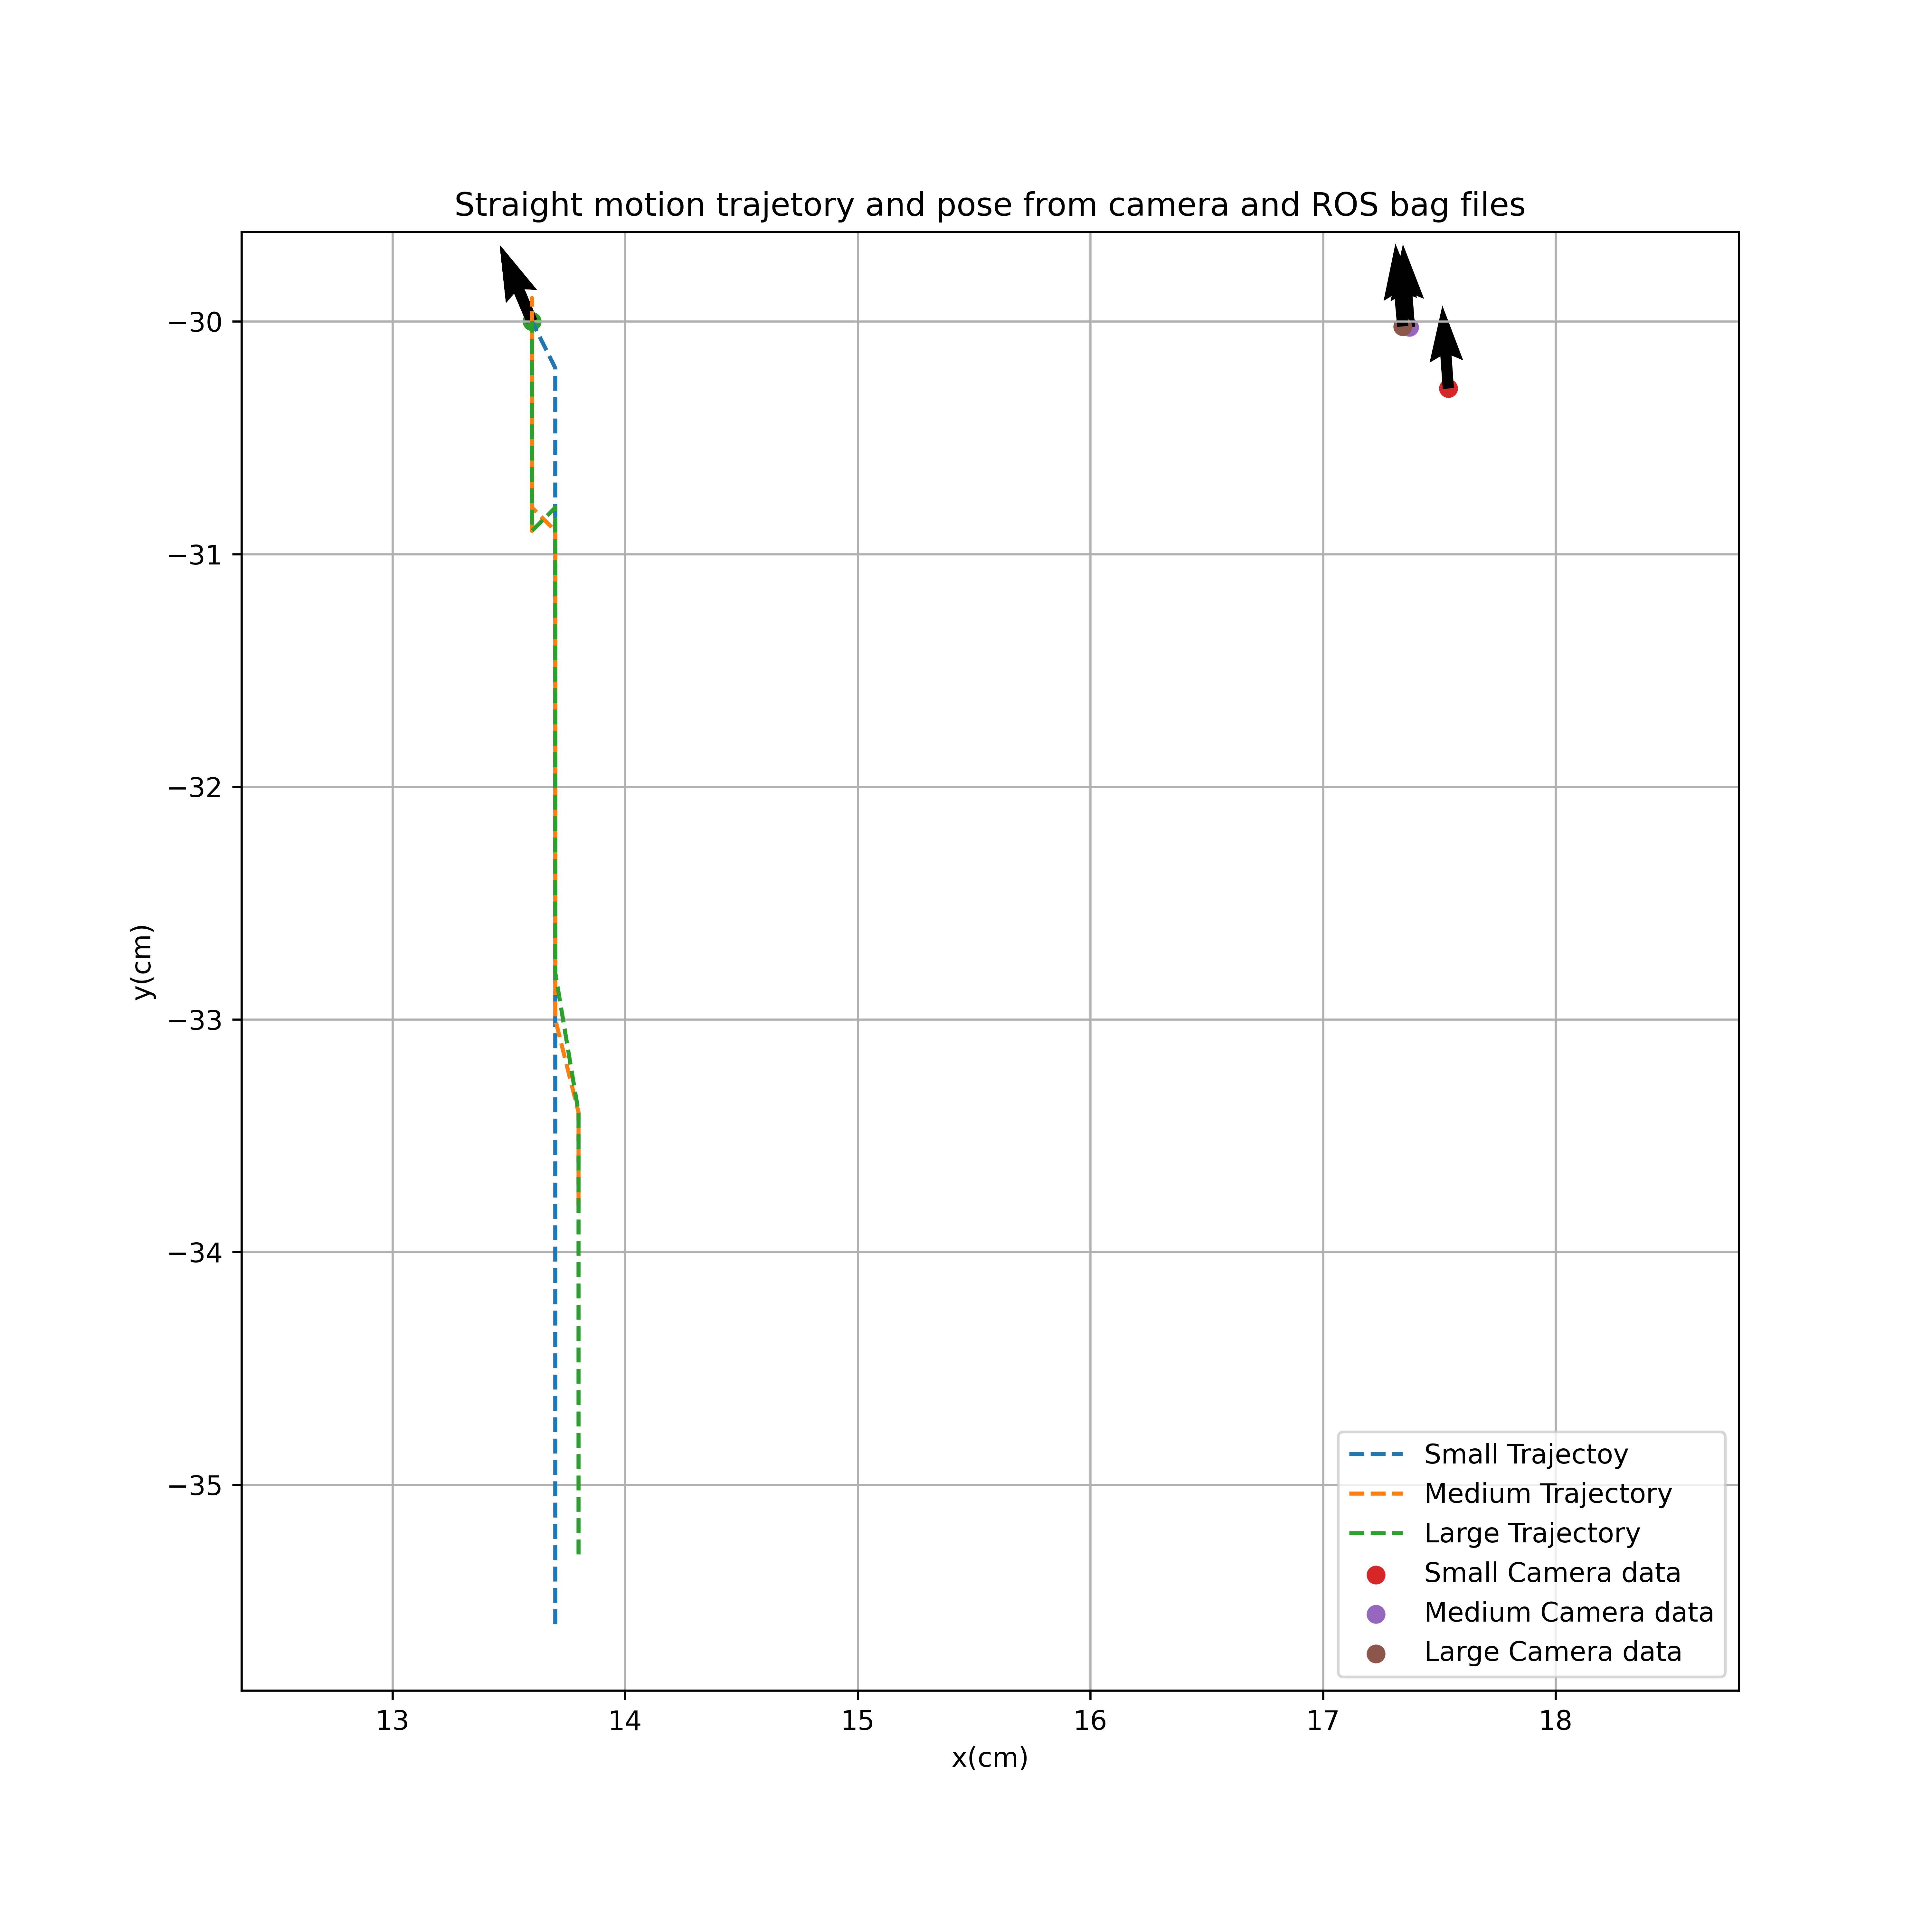
\includegraphics[width=\textwidth]{"images/experiment_5/Straight_motion_trajectory_camera.png"}
            \caption{{Straight Motion End effector poses and trajectory}}
            \label{fig:exp05-Straight Motion End effector poses and trajectory}
        \end{figure}
        
    
    \begin{figure}[H] 
            \centering 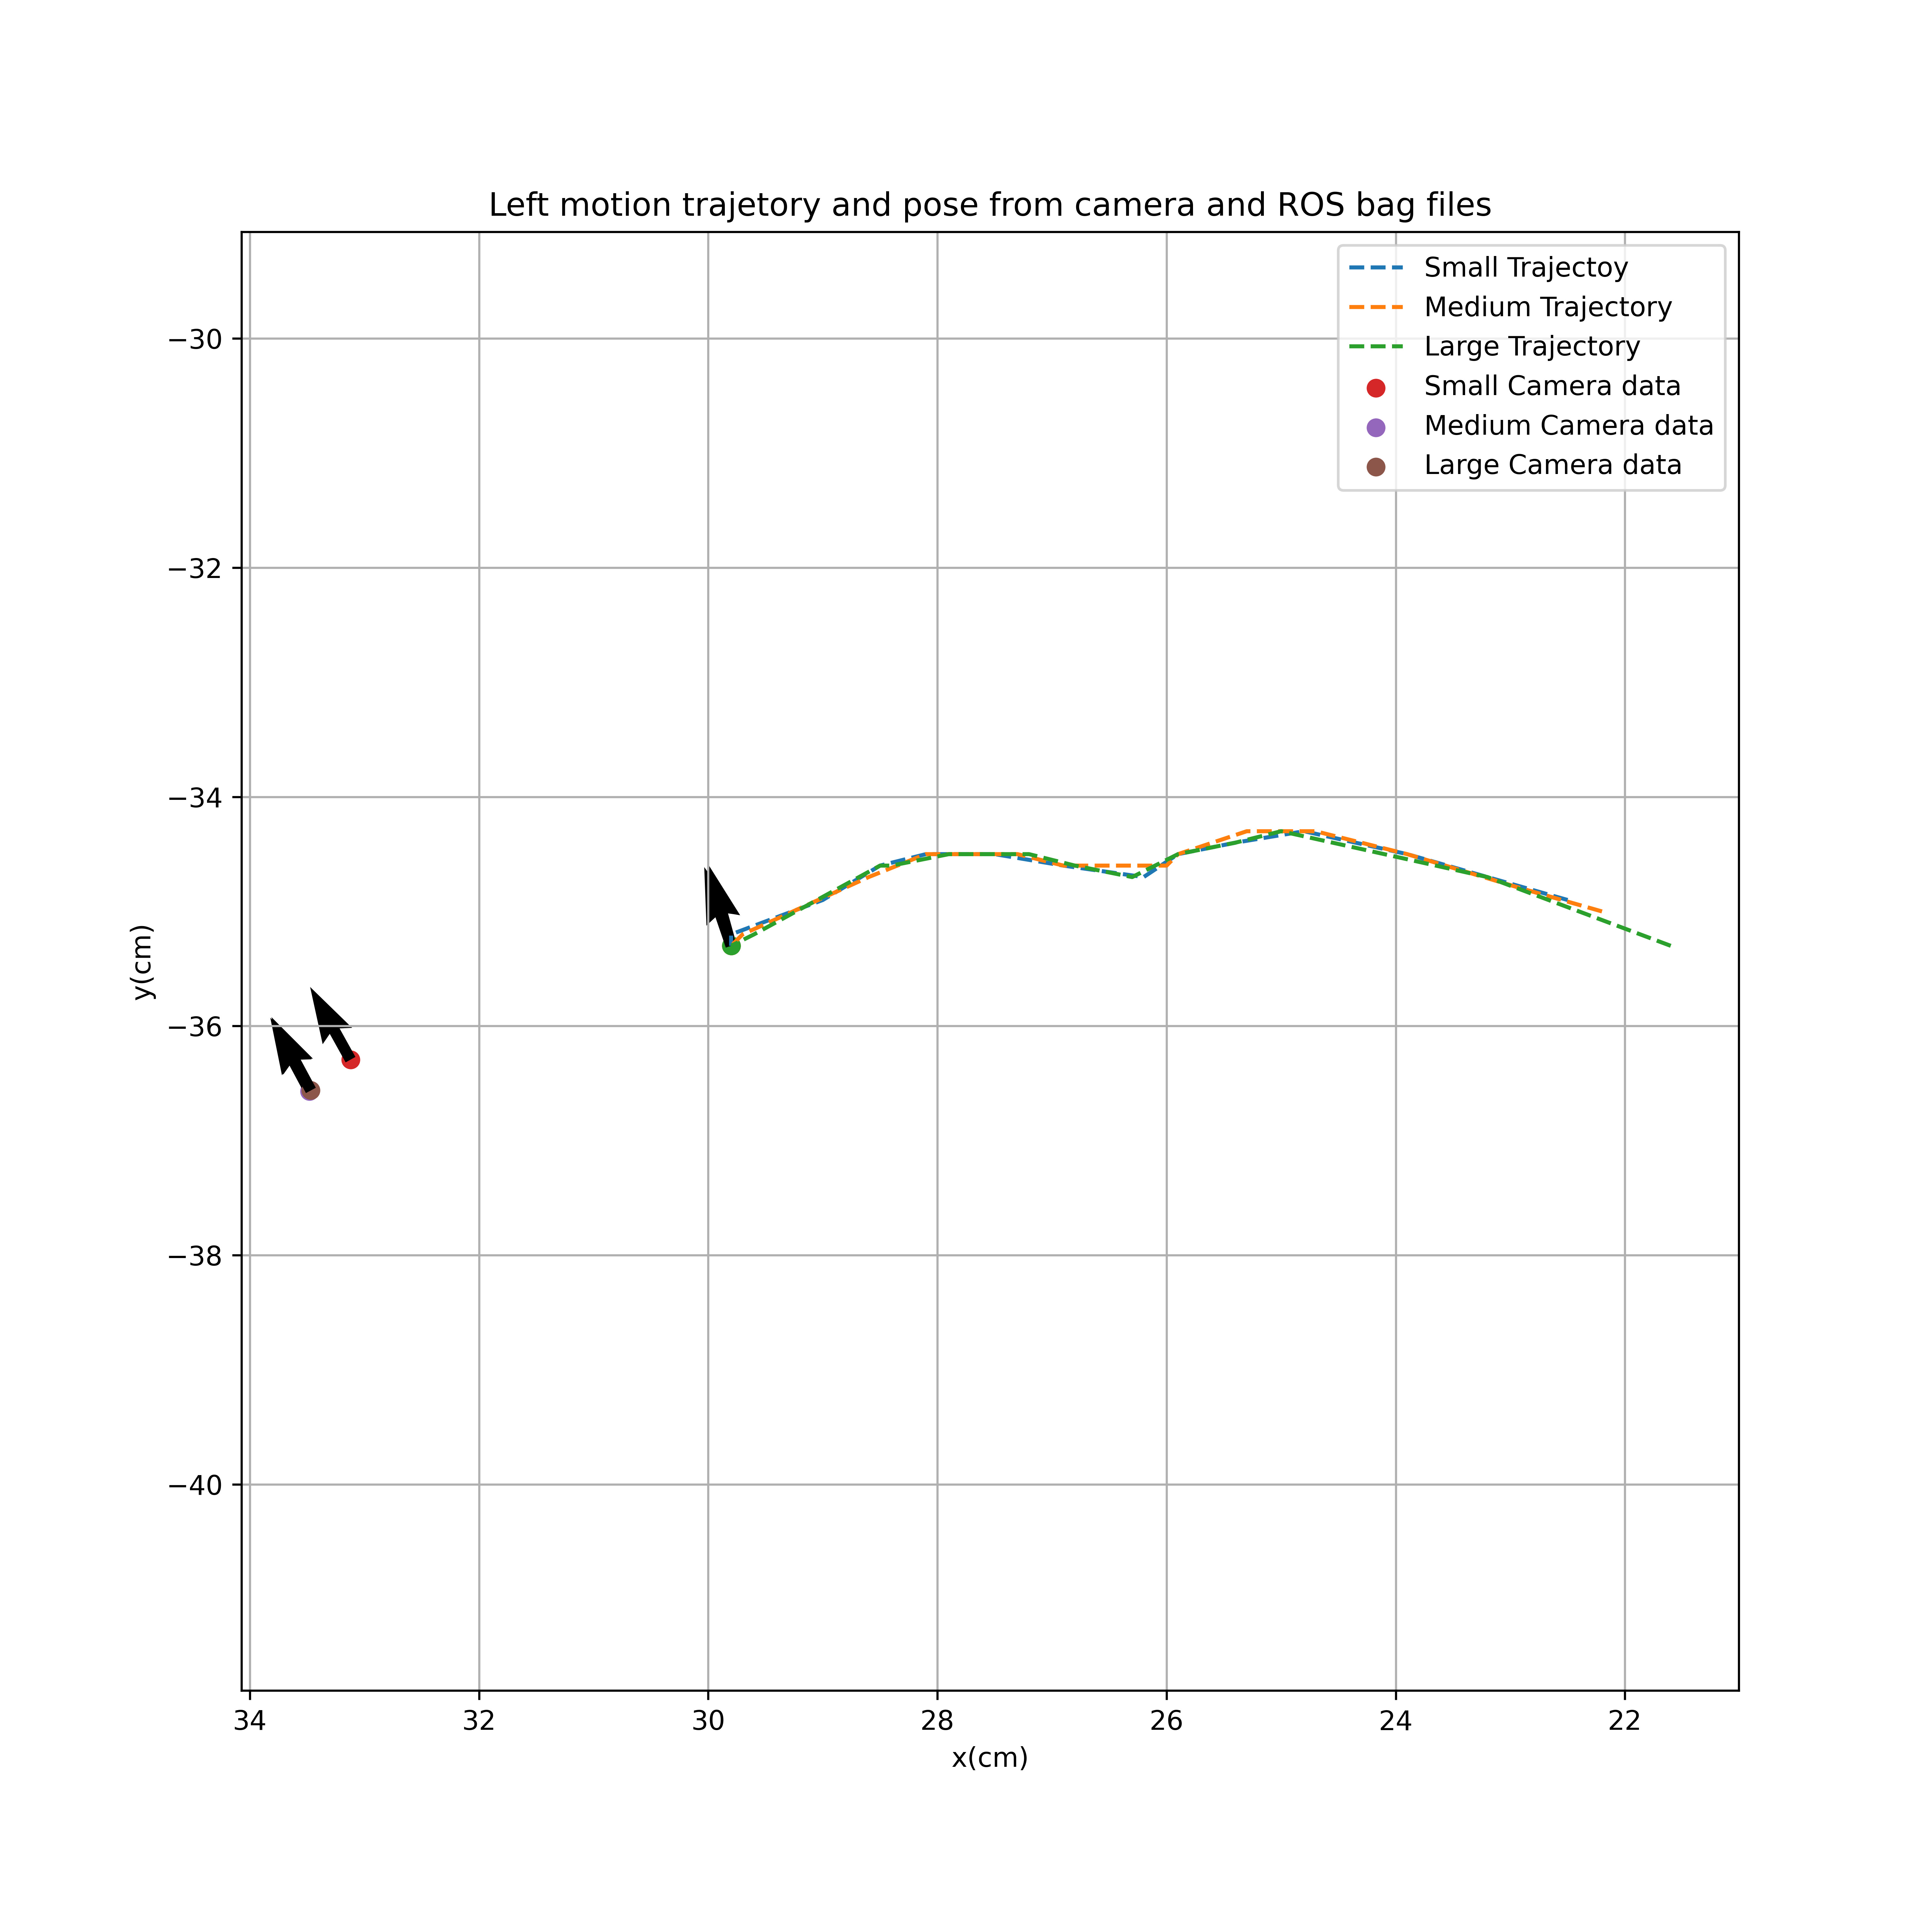
\includegraphics[width=\textwidth]{"images/experiment_5/Left_motion_trajectory_camera.png"}
            \caption{{Left Motion End effector poses and trajectory}}
            \label{fig:exp05-Left Motion End effector poses and trajectory}
        \end{figure}
        
    
    \begin{figure}[H] 
            \centering 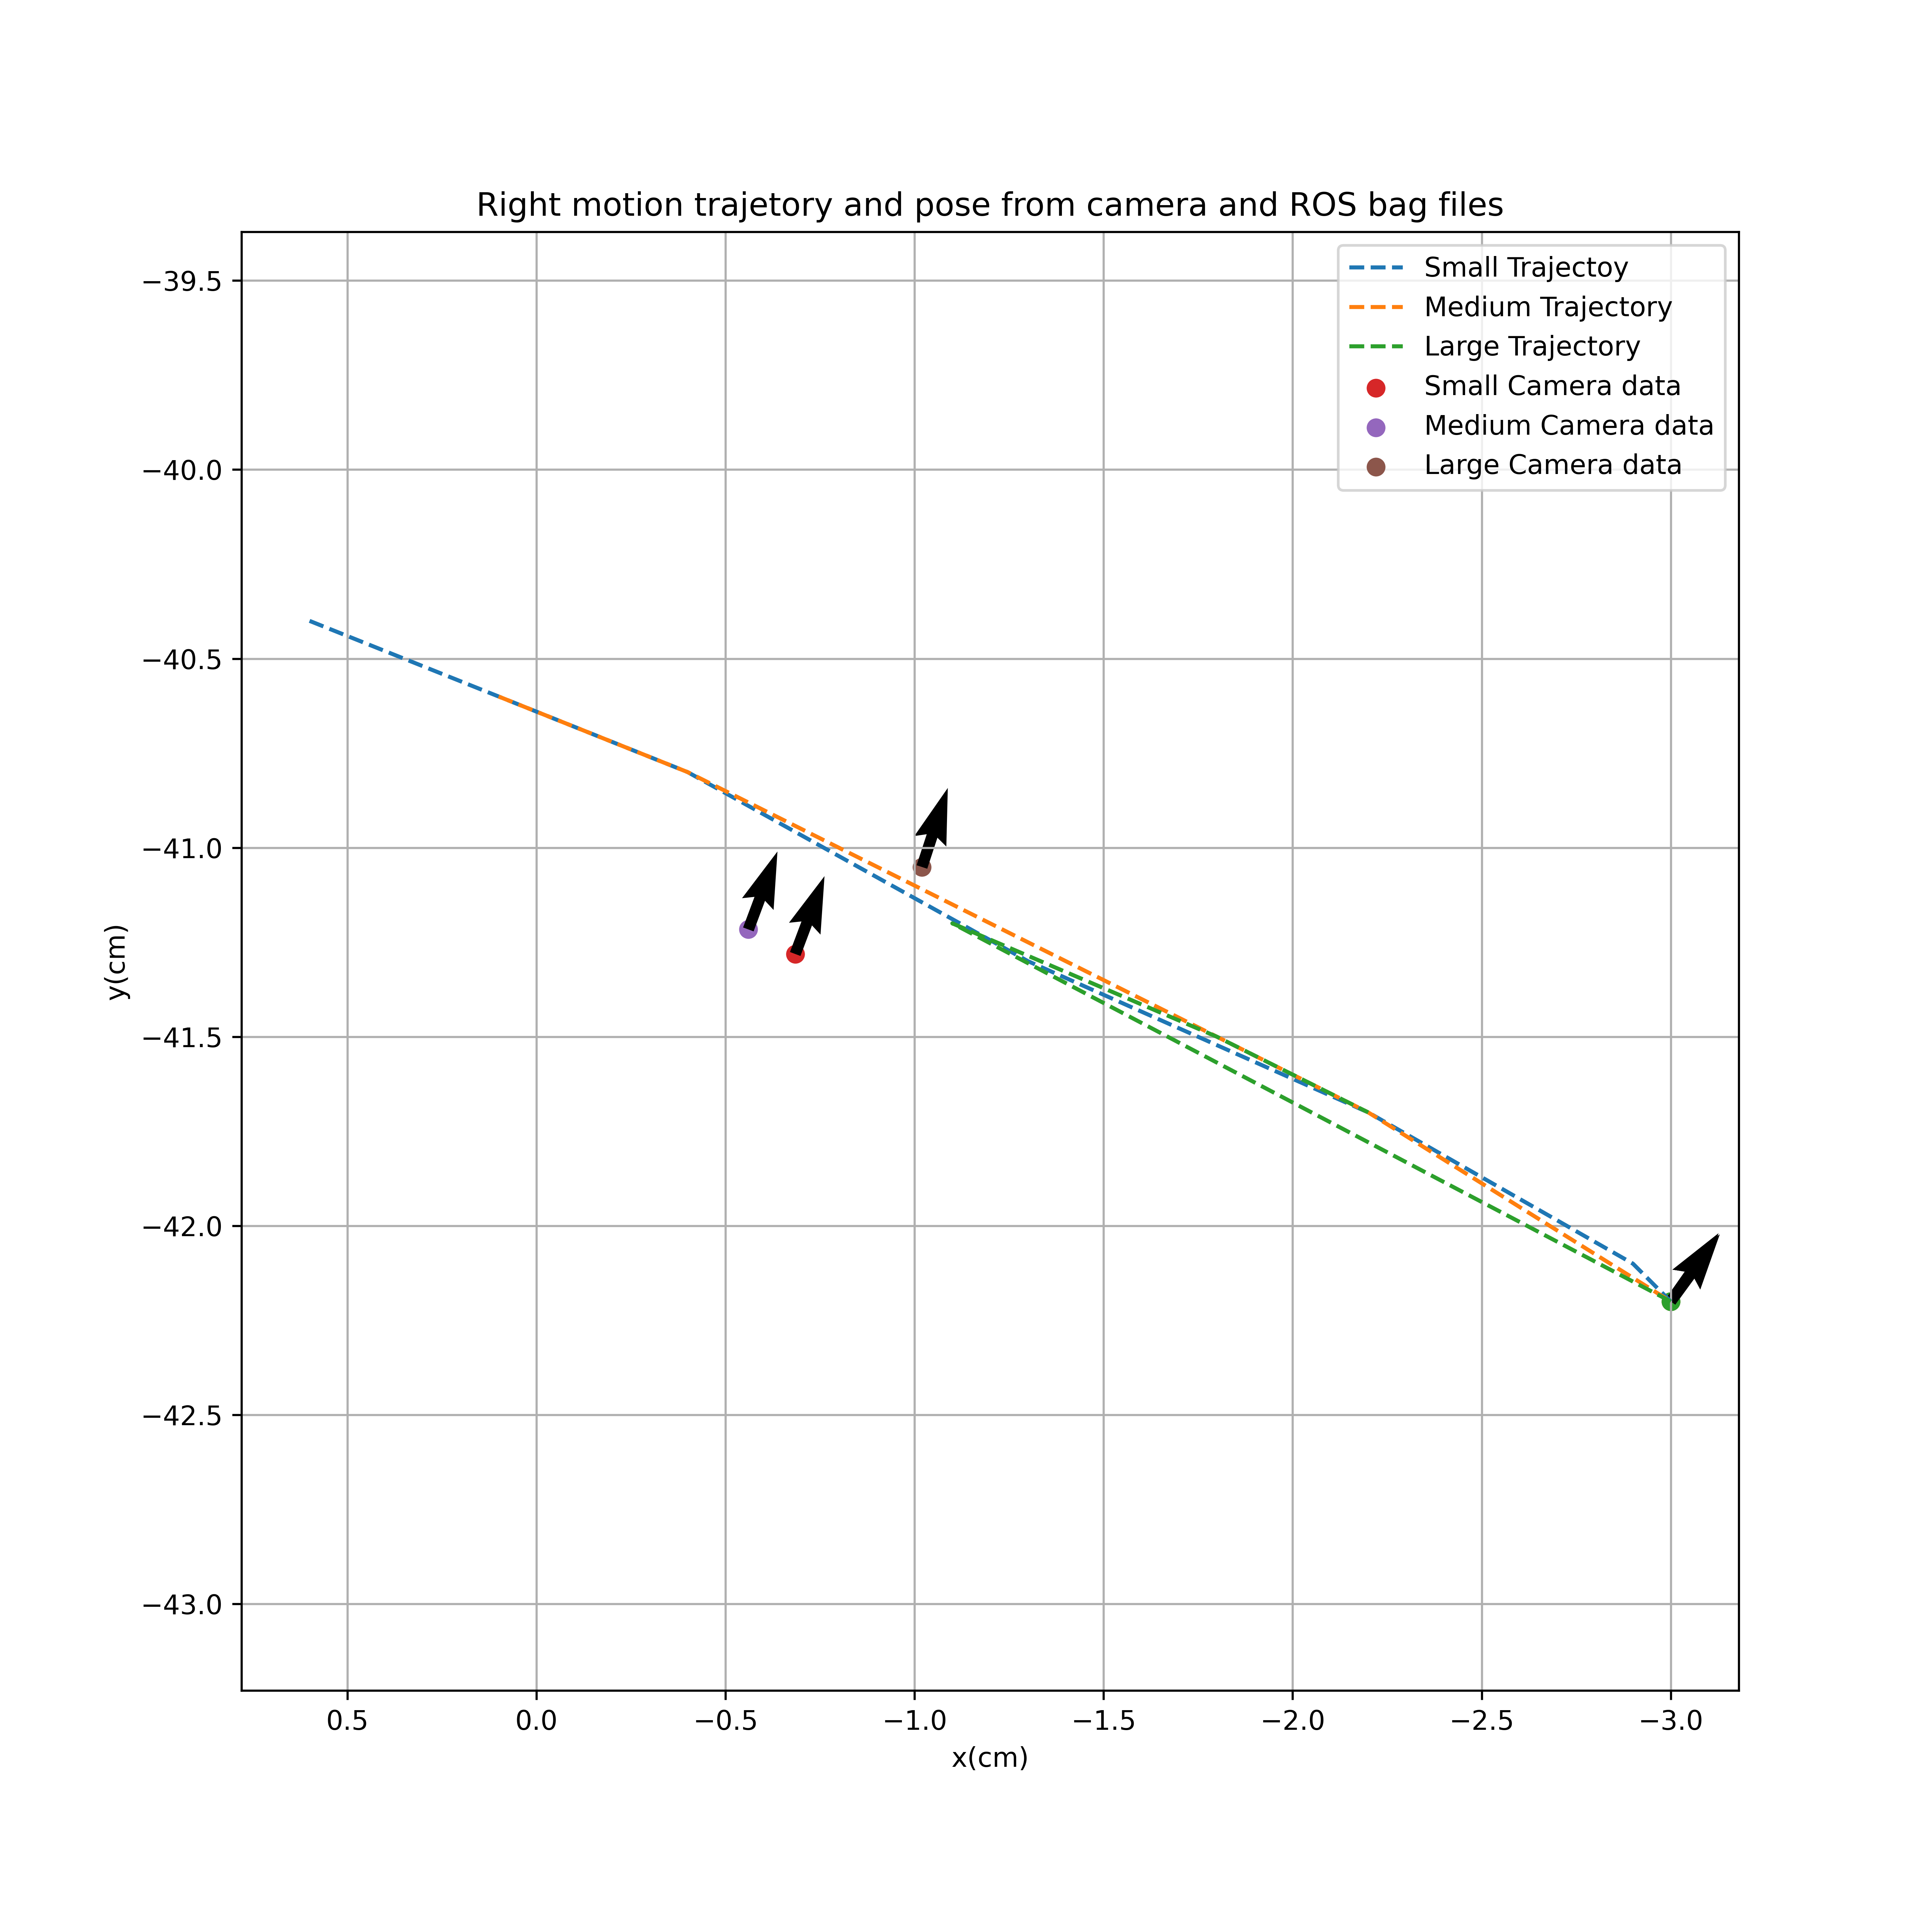
\includegraphics[width=0.9\textwidth]{"images/experiment_5/Right_motion_trajectory_camera.png"}
            \caption{{Right Motion End effector poses and trajectory}}
            \label{fig:exp05-Right MotionEnd effector poses and trajectory}
        \end{figure}
    
    %000000000000000000000000000000000000000000000000000000000000000000000000000000000000%
    

    
    
\end{document}
